\documentclass[./dissertation.tex]{subfiles}

\part{Scientific Contributions}
\chapter{Basic Hardware Components}
\section{Introduction}
In the context of new applications for autonomous mobility, digital components a required to reach high levels of functional safety performances. This level of assurance is necessary to supply safely the computational power and advanced processing required by those applications. It is therefore necessary for digital SoCs safety engineers to be able to demonstrate thru advanced provable methods the achieved reliability of their system and counter measures.
%Safety is also included in components requirements. Issues around implemented functionalities require high level of reliability. Applications don’t tolerate any errors. 

Similarly to complex electomecanical systems, it is difficult to predict the failure modes of a complex SoC which exhibits an almost infinite state space (in the order of $2^n$, {\it n} is the number of sequential elements, reaching ten's of thousands easily) and distributed-systems characteristics: numerous independents sub-systems operating and communicating asynchronously.

Digital systems are subject to two kind of errors, {\it permanent} which are created by destructive or aging effects, and {\it transient} \cite{Baumann_2005} created by particle impacts such as thermal neutrons at ground level or solar wind in low and high earth orbits \cite{DBLP:journals/ibmrd/ZieglerS96}\cite{8368564}. Permanent effects shows in the form of a permanent stuck to an electrical value ('0' or '1' logic value) and can occurs on any digital element (combinational logic, i.e. {\it logic gate} or sequential element, i.e. {\it flip-flops}). So do transient faults, also called {\it soft errors}, but with different, non-permanent, effects on logic or sequential elements. Transient faults on logic gates are called {\it Single Event Transient} (SET) \cite{Karnik2004CharacterizationOS} and are particularly dangerous on clock trees and reset trees (which distributes the clock and reset signals through the chip using trees of {\it buffers}) of SoCs as their effect, that has the form of a glitch, is to reset or desynchronize the sequencing of a sub-part of the system. Transient faults on sequential elements (memories or flip-flops) only invert the value of the element which will retain the faulty value until overwritten by a new value. They are called {\it Single Event Upset} (SEU) and are the main cause of safety goals violations in digital SoCs \cite{Mukherjee_2005}.

However, digital system exhibit a natural resistance to soft errors and most of them have no functional effect while a small proportion of them ($\approx 10\%$ of them in a standard 5-stages processor \cite{4358223, Mukherjee03asystematic}) will lead to system execution failure. FMEDA analysis \cite{4211846}, targeting goals such as ISO26262 automotive safety norm \cite{iso26262} certification will consist in quantifying those failure modes, proving the effectiveness of counter measures and absence of safety goals violation.
An effective solution consists in submitting the system to faults, by simulation or under radiation beam, therefore stressing it and provoking intentionally dysfunctional behaviors. Those 'out of trajectory' behaviors can then be recorded, analysed and used for FMEDA analysis in the certification process. However, both methods are costly both in term of engineering setup needed and cost: fault injection of a full SoC requires a complex setup, test suite and costly hardware emulator while radiation test requires an acquisition system, a test setup and access to costly and constrained radiation facilities, Both have the disadvantage to require, the full SoC gate netlist (fault injection \cite{Wang_2005}) or silicon (irradiation \cite{6861096}). Also, both methods can be classified as experimental as it is a verification 'by observation' of the resilience of the system to faults. No proof, except statistical confidence is made on the extracted faults metrics.

In this work, we aim to assess the capability of Model-Based Safety Assessment methods to build the dysfunctional model of a digital SoC from its subsystems and perform the currently hand-made FMEDA of the full system automatically. We expect the methods to be able to quantify globally the system safety metrics more accurately than with hand-made spreadsheets which only basically multiply probabilities. Automatic failure analysis such as fault trees extraction, fault sequences leading to unwanted events are also expected to be of great help during the certification process. The problem to solve is then to extract and build the required dysfunctional models of the different subsystems of the SoC and to properly expose the failure modes  in the constructed models to be able to use existing model composition frameworks.

%. MBSA describes architecture at system level and implement a failure propagation model. Model exploitation algorithms allow deducing combinations of failures leading to feared events and quantifying effects apparition probabilities. 

The document is organized as follow: we first present the system used as example and how fault injection is used to expose dysfunctional behaviors and extract a model. The chosen approach is then detailed reminding generic principles before explaining specific mechanisms put in place to model digital system. Finally, the document details fault injection campaign post-processing methods and obtained results. We compare composition results with fault injection performed on the full system used as a reference.


\section{State-of-the-Art}
\label{sec:sota}
\subsection{Probabilistic Methods in Digital Systems Safety}
Probabilistic methods \cite{5724504} \cite{Torras} have been developed to estimate propagation and masking rates of errors in gate netlists. Such approaches, restricted to combinational logic provide an helper to estimate certain metrics ($\lambda_{spf}$, i.e. {\it Dangerous Undetected} by a safety mechanism faults \cite{iso26262-acronyms}) required in ISO26262, but are far from being able to provide metrics even at the sequential block level. Likewise, industrial formal proof tools \cite{jaspergold} \cite{yeung-2018} are able to compute such metrics by using formal methods.

Methods like FIDES \cite{fides} \cite{FIDES_fault_tree} targets Commercial Off-the-Shelf (COTS) based Electronic Control Unit (ECU), with components failure rates extracted from available reliability databases. It takes into account systematic or aging failures but not transient effects such as soft-errors.
%limited to small designs even though they are able to perform safety related proofs such as proving absence of unwanted behavior in the presence of faults.

\subsection{Formal Methods in Digital Systems Safety}

Formal methods \cite{Brayton1996VISAS, Brayton2010ABCAA} are mostly used on unitary blocks or functionalities to prove assertions (i.e. properties) expressed in linear \cite{SVA} or branching \cite{EMERSON1980} timing logic. When applied to safety, it comes to proving absence of safety goals violations that are expressed as assertions on outputs in the presence of faults. Tools like \cite{jaspergold}\cite{yeung-2018} are able to compute, given a nelist of logic gates and flip-flops and an initial state, the cone of influence of flip-flops or gates and whether a fault in such elements can propagate to a given output. Such structural analysis can perform {\it Out-of-Cone-of-Influence} ({\it COI}) fault analysis allowing to classify a fault as {\it safe} when it cannot reach a given output. Activation analysis determine whether a fault injected on a specific node can be activated. Propagatability analysis determine if an activated fault in a COI can propagate to a strobed output and detection analysis determines if a fault will (always) be propagated and detected at the checker output. Such analysis can reveal what logic is covered by a safety mechanism or not. However, no formal methods is able to address such safety properties at SoC level.

%The second analysis such tools can do is relevant to safety mechanisms (blocks checking/correcting the behavior such as error correcting code on memories) and proving ...DAMIANO
%The concept behind formal verification is the 
%when a simulation is launched, an initial and a final state are connected thought a certain number of states belonging to the DUT FSM. This number of state is proportional to the coverage of the Test Bench used to exercise the DUT.
%Given a list of constraints, for instance on the value that a certain signal can take, it is possible to theoretically limit the working space of that signal. What the Formal Verification tools are able to do is to exercise the DUT while taking care of those constraints, raising exceptions if during the execution one of those limits is infringed, voiding the formal verification.
%Even if there exist tools for the actual verification, the set of signals and their constraints is still chosen by the designer and formalized in SystemVerilog.
%Is it possible to summarize the pros and cons of the formal verification procedure and its tools like \cite{jaspergold}\cite{ONESPIN} follows
%\begin{enumerate}
%    \item The main pros is that in functional verification only one path or a restricted set of paths while in the formal verification, ideally, all the possible ones
%    \item On the other hand the process of formal verification is much heavier in therms of licenses and computational power needed.
%\end{enumerate}

\subsection{Altarica} \label{Altarica}
Functional safety objective is to identify the most probable failure combinations leading to a feared event. Model-Based Safety Analysis performs safety analysis by building dysfunctional models for each block of the considered system and using formal methods to combine and extract failure modes at the system level \cite{mortada-imbsa-2014}. MBSA introduces the use of high level modeling languages dedicated to functional safety analysis \cite{Prosvirnova} \cite{arnold} \cite{bozzano-avocs-2010}. It allows extending classical methods such as FMEA or fault trees. These languages help capture system dynamics and how failures propagate inside it. Moreover, models support structural modeling allowing identifying and locating induced effects of a failure inside the architecture. 

Altarica Dataflow (Fig. \ref{altarica-dataflow}) is an event-driven asynchronous language that implements discrete variables with a finite number of values, leading to a finite number of combinations of state values and propagated flows, allowing theoretically to cover the entire system state space. AltaRica Dataflow is at the core of several Reliability, Availability, Maintainability and Safety (RAMS) environments: Cecilia OCAS (Dassault Aviation), SimfiaNeo (Airbus Protect), and Safety Designer (Dassault Syst\`emes)


\begin{figure}[h]

\centering






\tikzset{every picture/.style={line width=0.75pt}} %set default line width to 0.75pt        

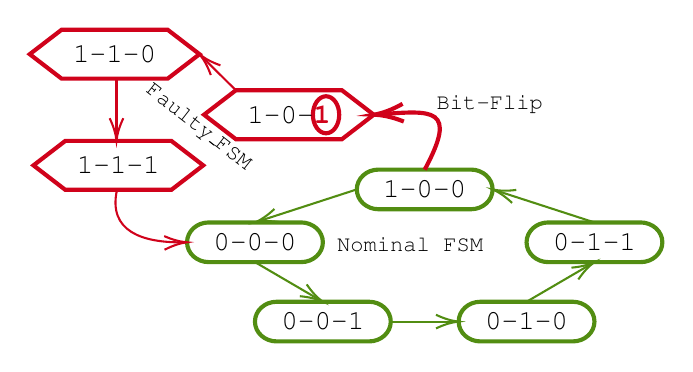
\begin{tikzpicture}[x=0.75pt,y=0.75pt,yscale=-1,xscale=1]
%uncomment if require: \path (0,300); %set diagram left start at 0, and has height of 300

%Flowchart: Terminator [id:dp9084086847868367] 
\draw  [color={rgb, 255:red, 82; green, 141; blue, 18 }  ,draw opacity=1 ][line width=1.5]  (137.18,177.49) -- (181.67,177.49) .. controls (187.46,177.49) and (192.14,181.77) .. (192.14,187.05) .. controls (192.14,192.32) and (187.46,196.6) .. (181.67,196.6) -- (137.18,196.6) .. controls (131.4,196.6) and (126.71,192.32) .. (126.71,187.05) .. controls (126.71,181.77) and (131.4,177.49) .. (137.18,177.49) -- cycle ;
%Flowchart: Terminator [id:dp921126991920133] 
\draw  [color={rgb, 255:red, 82; green, 141; blue, 18 }  ,draw opacity=1 ][line width=1.5]  (235.33,177.49) -- (279.82,177.49) .. controls (285.6,177.49) and (290.29,181.77) .. (290.29,187.05) .. controls (290.29,192.32) and (285.6,196.6) .. (279.82,196.6) -- (235.33,196.6) .. controls (229.54,196.6) and (224.86,192.32) .. (224.86,187.05) .. controls (224.86,181.77) and (229.54,177.49) .. (235.33,177.49) -- cycle ;
%Flowchart: Terminator [id:dp9486811695622979] 
\draw  [color={rgb, 255:red, 82; green, 141; blue, 18 }  ,draw opacity=1 ][line width=1.5]  (268.04,139.28) -- (312.53,139.28) .. controls (318.31,139.28) and (323,143.56) .. (323,148.84) .. controls (323,154.11) and (318.31,158.39) .. (312.53,158.39) -- (268.04,158.39) .. controls (262.26,158.39) and (257.57,154.11) .. (257.57,148.84) .. controls (257.57,143.56) and (262.26,139.28) .. (268.04,139.28) -- cycle ;
%Flowchart: Terminator [id:dp9555553349711161] 
\draw  [color={rgb, 255:red, 82; green, 141; blue, 18 }  ,draw opacity=1 ][line width=1.5]  (186.25,113.81) -- (230.75,113.81) .. controls (236.53,113.81) and (241.21,118.09) .. (241.21,123.36) .. controls (241.21,128.64) and (236.53,132.92) .. (230.75,132.92) -- (186.25,132.92) .. controls (180.47,132.92) and (175.79,128.64) .. (175.79,123.36) .. controls (175.79,118.09) and (180.47,113.81) .. (186.25,113.81) -- cycle ;
%Flowchart: Terminator [id:dp500677861210465] 
\draw  [color={rgb, 255:red, 82; green, 141; blue, 18 }  ,draw opacity=1 ][line width=1.5]  (104.47,139.28) -- (148.96,139.28) .. controls (154.74,139.28) and (159.43,143.56) .. (159.43,148.84) .. controls (159.43,154.11) and (154.74,158.39) .. (148.96,158.39) -- (104.47,158.39) .. controls (98.69,158.39) and (94,154.11) .. (94,148.84) .. controls (94,143.56) and (98.69,139.28) .. (104.47,139.28) -- cycle ;
%Flowchart: Preparation [id:dp3607152634107744] 
\draw  [color={rgb, 255:red, 208; green, 2; blue, 27 }  ,draw opacity=1 ][line width=1.5]  (102.18,87.38) -- (117.51,75.6) -- (168.63,75.6) -- (183.96,87.38) -- (168.63,99.16) -- (117.51,99.16) -- cycle ;
%Straight Lines [id:da8805114399762077] 
\draw [color={rgb, 255:red, 82; green, 141; blue, 18 }  ,draw opacity=1 ][line width=0.75]    (192.14,187.05) -- (222.86,187.05) ;
\draw [shift={(224.86,187.05)}, rotate = 180] [color={rgb, 255:red, 82; green, 141; blue, 18 }  ,draw opacity=1 ][line width=0.75]    (10.93,-3.29) .. controls (6.95,-1.4) and (3.31,-0.3) .. (0,0) .. controls (3.31,0.3) and (6.95,1.4) .. (10.93,3.29)   ;
%Straight Lines [id:da6495626037090436] 
\draw [color={rgb, 255:red, 82; green, 141; blue, 18 }  ,draw opacity=1 ][line width=0.75]    (257.57,177.49) -- (288.56,159.4) ;
\draw [shift={(290.29,158.39)}, rotate = 509.71] [color={rgb, 255:red, 82; green, 141; blue, 18 }  ,draw opacity=1 ][line width=0.75]    (10.93,-3.29) .. controls (6.95,-1.4) and (3.31,-0.3) .. (0,0) .. controls (3.31,0.3) and (6.95,1.4) .. (10.93,3.29)   ;
%Straight Lines [id:da832753655405839] 
\draw [color={rgb, 255:red, 82; green, 141; blue, 18 }  ,draw opacity=1 ][line width=0.75]    (290.29,139.28) -- (243.12,123.98) ;
\draw [shift={(241.21,123.36)}, rotate = 377.98] [color={rgb, 255:red, 82; green, 141; blue, 18 }  ,draw opacity=1 ][line width=0.75]    (10.93,-3.29) .. controls (6.95,-1.4) and (3.31,-0.3) .. (0,0) .. controls (3.31,0.3) and (6.95,1.4) .. (10.93,3.29)   ;
%Straight Lines [id:da7173988733392529] 
\draw [color={rgb, 255:red, 82; green, 141; blue, 18 }  ,draw opacity=1 ]   (175.79,123.36) -- (128.62,138.67) ;
\draw [shift={(126.71,139.28)}, rotate = 342.02] [color={rgb, 255:red, 82; green, 141; blue, 18 }  ,draw opacity=1 ][line width=0.75]    (10.93,-3.29) .. controls (6.95,-1.4) and (3.31,-0.3) .. (0,0) .. controls (3.31,0.3) and (6.95,1.4) .. (10.93,3.29)   ;
%Straight Lines [id:da4444324956160115] 
\draw [color={rgb, 255:red, 82; green, 141; blue, 18 }  ,draw opacity=1 ][line width=0.75]    (126.71,158.39) -- (157.7,176.49) ;
\draw [shift={(159.43,177.49)}, rotate = 210.29] [color={rgb, 255:red, 82; green, 141; blue, 18 }  ,draw opacity=1 ][line width=0.75]    (10.93,-3.29) .. controls (6.95,-1.4) and (3.31,-0.3) .. (0,0) .. controls (3.31,0.3) and (6.95,1.4) .. (10.93,3.29)   ;
%Curve Lines [id:da8286337939248241] 
\draw [color={rgb, 255:red, 208; green, 2; blue, 27 }  ,draw opacity=1 ][line width=1.5]    (208.5,113.81) .. controls (224.68,83.7) and (212.3,85.31) .. (186.79,87.18) ;
\draw [shift={(183.96,87.38)}, rotate = 356.01] [color={rgb, 255:red, 208; green, 2; blue, 27 }  ,draw opacity=1 ][line width=1.5]    (14.21,-4.28) .. controls (9.04,-1.82) and (4.3,-0.39) .. (0,0) .. controls (4.3,0.39) and (9.04,1.82) .. (14.21,4.28)   ;
%Shape: Ellipse [id:dp5162086532146974] 
\draw  [color={rgb, 255:red, 208; green, 2; blue, 27 }  ,draw opacity=1 ][line width=1.5]  (154.63,87.4) .. controls (154.63,82.48) and (157.47,78.48) .. (160.97,78.48) .. controls (164.47,78.48) and (167.31,82.48) .. (167.31,87.4) .. controls (167.31,92.32) and (164.47,96.32) .. (160.97,96.32) .. controls (157.47,96.32) and (154.63,92.32) .. (154.63,87.4) -- cycle ;
%Flowchart: Preparation [id:dp6863452696605052] 
\draw  [color={rgb, 255:red, 208; green, 2; blue, 27 }  ,draw opacity=1 ][line width=1.5]  (18.21,58.22) -- (33.55,46.44) -- (84.67,46.44) -- (100,58.22) -- (84.67,70) -- (33.55,70) -- cycle ;
%Flowchart: Preparation [id:dp4786296734641169] 
\draw  [color={rgb, 255:red, 208; green, 2; blue, 27 }  ,draw opacity=1 ][line width=1.5]  (20,111.78) -- (35.33,100) -- (86.45,100) -- (101.79,111.78) -- (86.45,123.56) -- (35.33,123.56) -- cycle ;
%Straight Lines [id:da32998830369668064] 
\draw [color={rgb, 255:red, 208; green, 2; blue, 27 }  ,draw opacity=1 ]   (60,70) -- (60,98) ;
\draw [shift={(60,100)}, rotate = 270] [color={rgb, 255:red, 208; green, 2; blue, 27 }  ,draw opacity=1 ][line width=0.75]    (10.93,-3.29) .. controls (6.95,-1.4) and (3.31,-0.3) .. (0,0) .. controls (3.31,0.3) and (6.95,1.4) .. (10.93,3.29)   ;
%Straight Lines [id:da0480102553857773] 
\draw [color={rgb, 255:red, 208; green, 2; blue, 27 }  ,draw opacity=1 ]   (117.51,75.6) -- (101.42,59.63) ;
\draw [shift={(100,58.22)}, rotate = 404.78] [color={rgb, 255:red, 208; green, 2; blue, 27 }  ,draw opacity=1 ][line width=0.75]    (10.93,-3.29) .. controls (6.95,-1.4) and (3.31,-0.3) .. (0,0) .. controls (3.31,0.3) and (6.95,1.4) .. (10.93,3.29)   ;
%Curve Lines [id:da1070388681167187] 
\draw [color={rgb, 255:red, 208; green, 2; blue, 27 }  ,draw opacity=1 ]   (60.2,123.8) .. controls (55.93,143.59) and (72.36,149.07) .. (92.15,148.87) ;
\draw [shift={(94,148.84)}, rotate = 538.4300000000001] [color={rgb, 255:red, 208; green, 2; blue, 27 }  ,draw opacity=1 ][line width=0.75]    (10.93,-3.29) .. controls (6.95,-1.4) and (3.31,-0.3) .. (0,0) .. controls (3.31,0.3) and (6.95,1.4) .. (10.93,3.29)   ;

% Text Node
\draw (126.71,148.84) node   [align=left] {{\fontfamily{pcr}\selectfont 0-0-0}};
% Text Node
\draw (159.43,187.05) node   [align=left] {{\fontfamily{pcr}\selectfont 0-0-1}};
% Text Node
\draw (257.57,187.05) node   [align=left] {{\fontfamily{pcr}\selectfont 0-1-0}};
% Text Node
\draw (290.29,148.84) node   [align=left] {{\fontfamily{pcr}\selectfont 0-1-1}};
% Text Node
\draw (208.5,123.36) node   [align=left] {{\fontfamily{pcr}\selectfont 1-0-0}};
% Text Node
\draw (143.07,87.38) node   [align=left] {{\fontfamily{pcr}\selectfont 1-0-\textcolor[rgb]{0.82,0.01,0.11}{\textbf{1}}}};
% Text Node
\draw (212.76,76.15) node [anchor=north west][inner sep=0.75pt]  [font=\footnotesize] [align=left] {{\fontfamily{pcr}\selectfont Bit-Flip}};
% Text Node
\draw (164.76,144.55) node [anchor=north west][inner sep=0.75pt]  [font=\footnotesize] [align=left] {{\fontfamily{pcr}\selectfont Nominal FSM}};
% Text Node
\draw (59.11,58.22) node   [align=left] {{\fontfamily{pcr}\selectfont 1-1-0}};
% Text Node
\draw (60.89,111.78) node   [align=left] {{\fontfamily{pcr}\selectfont 1-1-1}};
% Text Node
\draw (77.68,68.96) node [anchor=north west][inner sep=0.75pt]  [font=\footnotesize,rotate=-38] [align=left] {{\fontfamily{pcr}\selectfont Faulty\_FSM}};



\end{tikzpicture}

\caption{Non Explicit State Exploration Example}
\label{counter}
\end{figure}


%AltaRica is a safety modeling dedicated language  belonging to that c. Version used on this project, commonly called DataFlow, relies on mode automata formalism. This choice has been done as it is the version with adequate tools for model post processing. Elementary nodes implement state-transition systems, state machines describing the set of states of a component and the set of transitions to reach those states. Nodes are linked by flows which propagate the value of a variable from one node to the other. It reproduces the functional architecture of the system. Transitions are associated to triggering events. Those events are parametrized by a probability law ruling their triggering.
%Functional safety objective is to identify the most probable failure combinations leading to a feared event. Failure appearance obeys to a probability law and failures can be qualified as rare. An event-driven asynchronous model as described by AltaRica language appears fully suited for this application. Moreover, DataFlow implements discrete variables with a finite number of values. Consequently, there exists a finite number of combinations of state values and propagated flows which allows theoretically to cover the entire system space state. This property is limited by combinatory explosion, forcing to choose the right level of discretization. This level is the right balance between model representativeness and processing performances. 
\begin{itemize}
\item {\it Variables}:
AltaRica variables are discrete and represents an enumerated finite set of values called its {\it domain}. Variable definition inside its domain is free. The variable can represent for example functional modes, dysfunctional status, message types \ldots .

Inside MBSA models, state variables are generally used to represent dysfunctional status with a default value as nominal behavior and a value for each degraded mode reached from any failure mode. Flow variables are generally to describe the type of data exchanged between components. This type can represent a functional value (e.g. instruction value) or a dysfunctional value (e.g. message status). It depends of the model level of detail. As flows are used to propagate failures, they can be described either by sending a status or a faulty value.

\item {\it Transitions}:
Transitions describe possible states changing values. Transitions are guarded by a condition allowing the transition to become fireable when true. A transition is associated with a triggering event and is fired when the event is triggered and the guard is true. In MBSA modeling, triggering events are used to represent failure modes. AltaRica allows to assign a probability law to an event, modeling the behavior of random failures or deterministic actions. The transition completion describes the effect of the failure mode on the component state. Guards can be enriched to restrict to describe conditional failures. For example, in a cold redundancy, some failures can’t happen when the component is off.

\item {\it Assertions}:
Assertion is the mechanism used to set outputs values of a node. Output values are a function of input values and internal state values. Assertion can be interpreted as a logical function describing a truth table assigning outputs according to each combination of inputs and internal state values. Combinations are described through Boolean expressions and imperative programming constructs such as {\it if-then-else} or {\it case}. 

Assertions are used to propagate failures from a faulty component to other blocks. Fault injected on the internal state is propagated to its output and then to others blocks. Depending of the granularity level of the model, assertions are manipulating either functional values or states.
%When everything is nominal, assertions contain the functional behavior of the system. 
\end{itemize}

\section{First Manual Application of FMEA on a SoC}
In order to fully undestand the challenges that performing the full FMEA process implies (as depicted in chapter MISSIN REF), the decision of fully implement the process on a selected SoC has been taken.
The SoC on choice has been the RISC-V based SoC developed in STMicroelectronics, in order to have full observability and have all the testing suite and reports of irradiation available. 
Figure \ref{scr1_rtl} shows the complexity of the entire system of choice $SCR1$, composed of two cores and several peripherals, each of those dedicated to a specific communication or testing function.  



\begin{figure}[H]
    \centering
    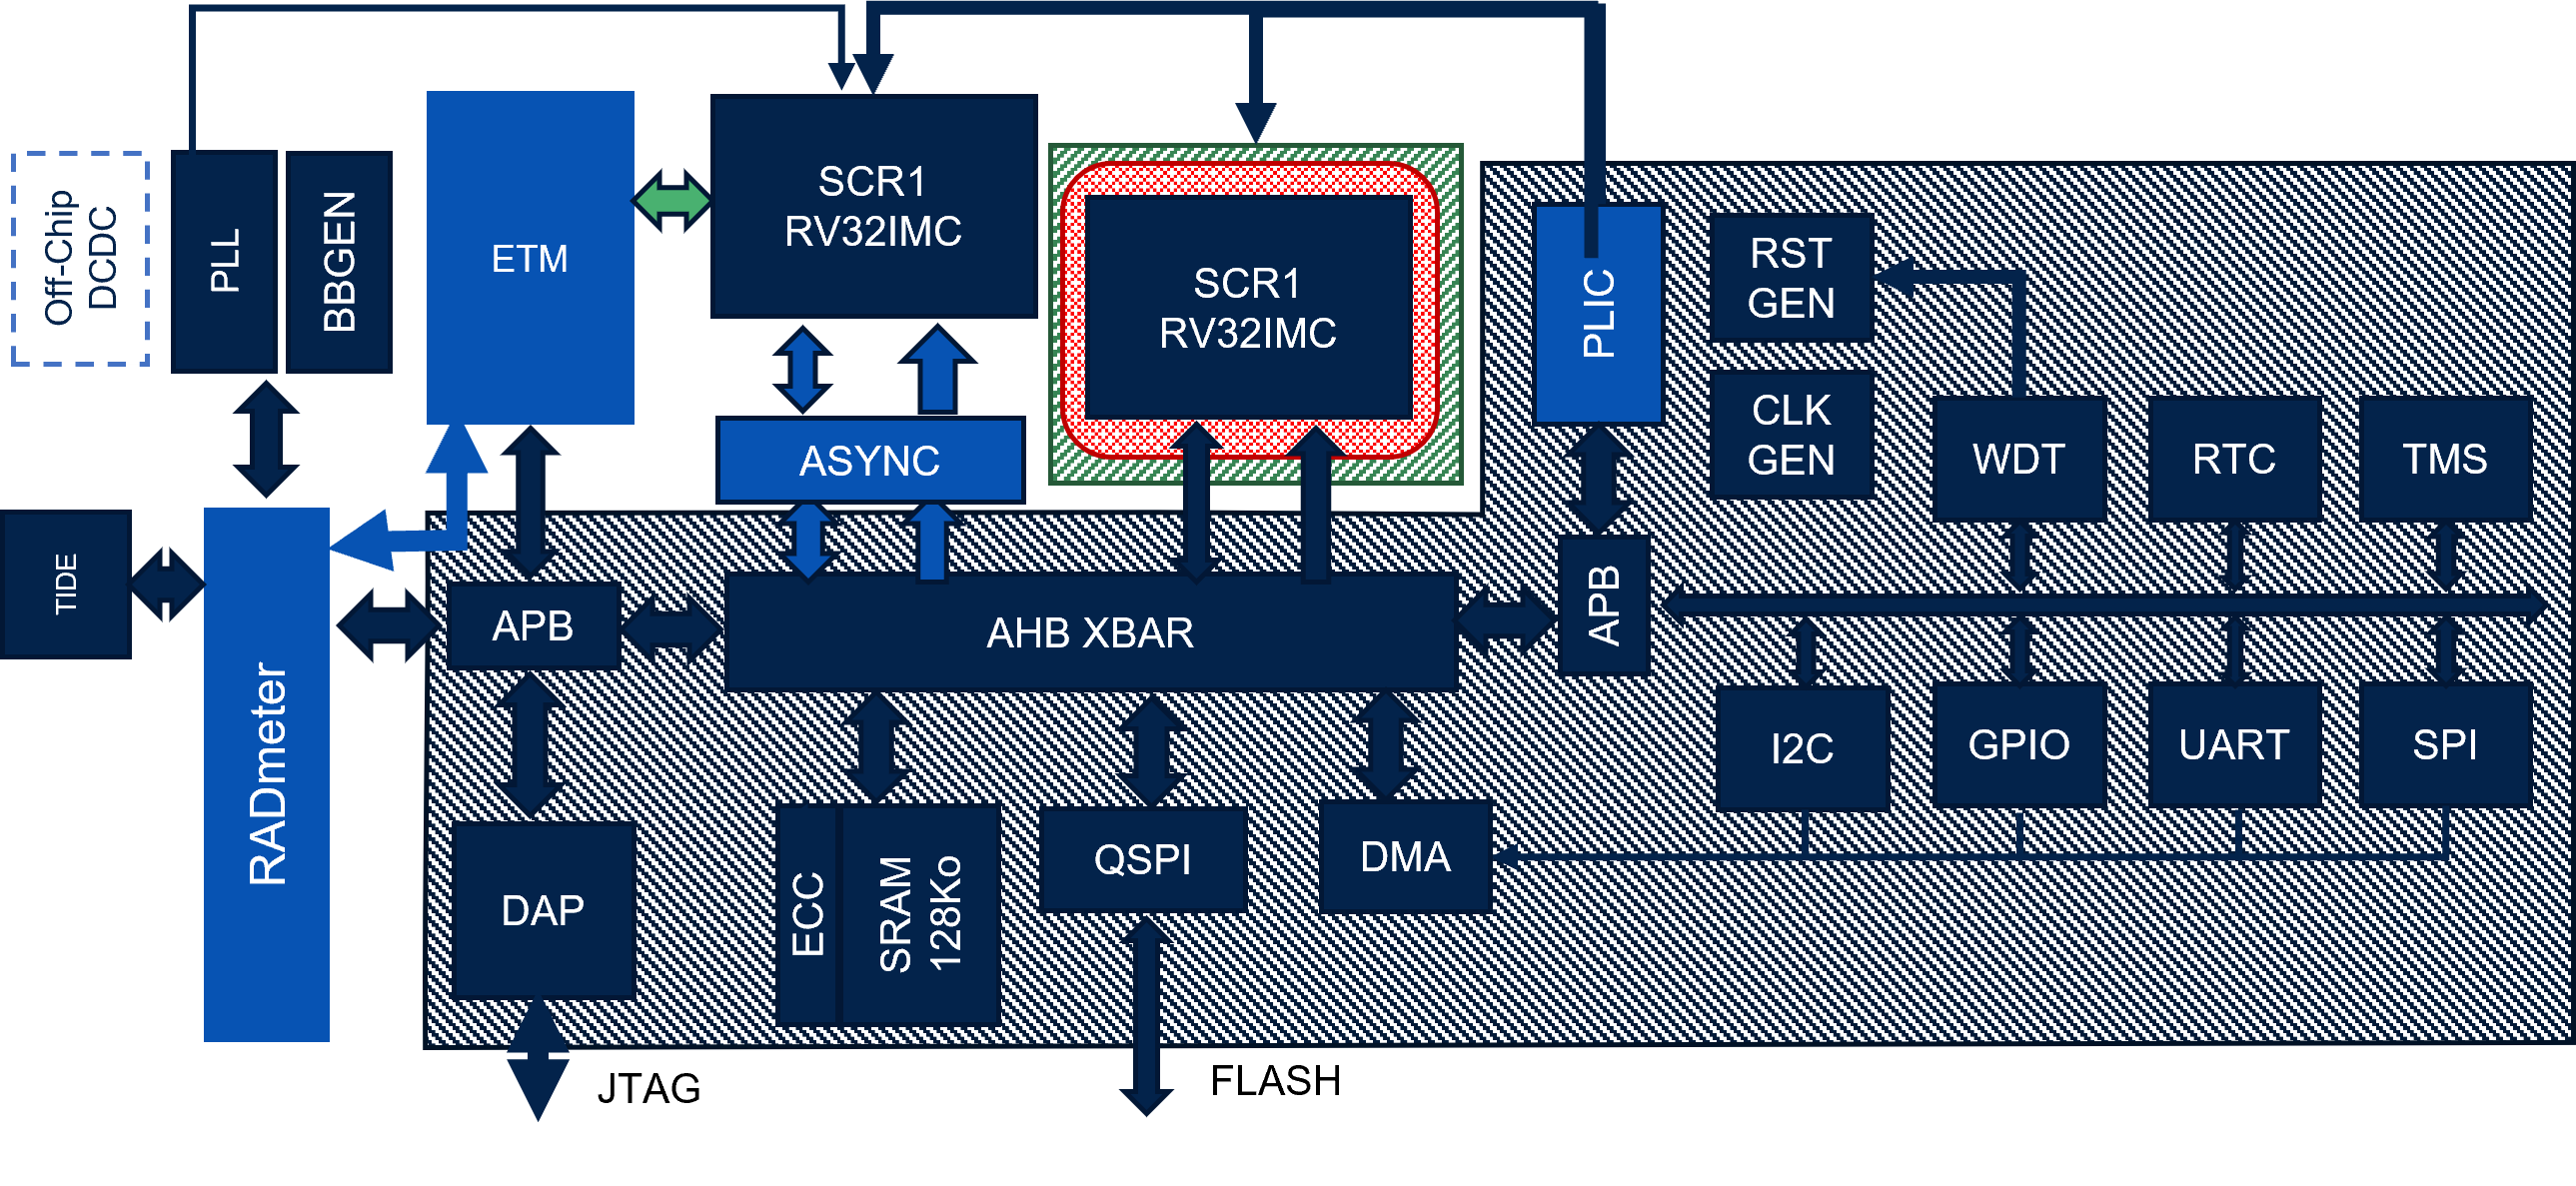
\includegraphics[width=\linewidth]{subfiles/imgs/scr1.png}
    \caption{\centering RTL Description of SCR1}
    \label{scr1_rtl}
\end{figure}

It has been clear since the beginning that the gratest obstacle to overcome was the definition of the internal blocks of the cores, together with their interconnections. There is where the FMEA process has started. There was the need to identify one of the two twin cores and decompose it manually in order to obtain a complete definition to then analyse the possible failure modes. Figure\ref{scr1_inputs} shows the beginning of the process, dictated by the identification of all the connections to peripherals that are established with the core of choice.

\begin{figure}[H]
    \centering
    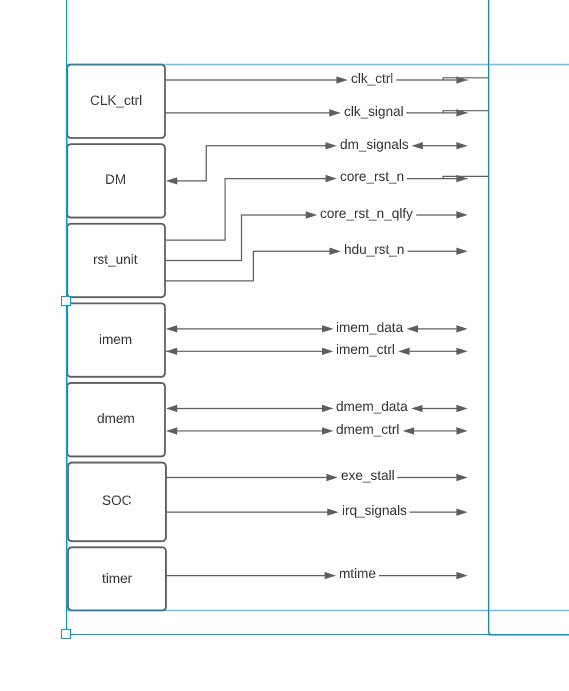
\includegraphics[width=\linewidth]{subfiles/imgs/pppp.png}
    \caption{\centering Inputs to the SoC}
    \label{scr1_inputs}
\end{figure}

That being the starting point, the work has proceeded with the definition of all the internal signals to all the sub-blocks of which the core is composed. This is a rather time consuming operation to be carried out manually, and it will be shown, one of the most prone to introduce human errors. Nevertheless it has been completed and the results are shown in Fig. \ref{scr1_blocks}, showing how complex the interconnections could be even in case of a high level description of the internal of the core.

\begin{figure}[H]
    \centering
    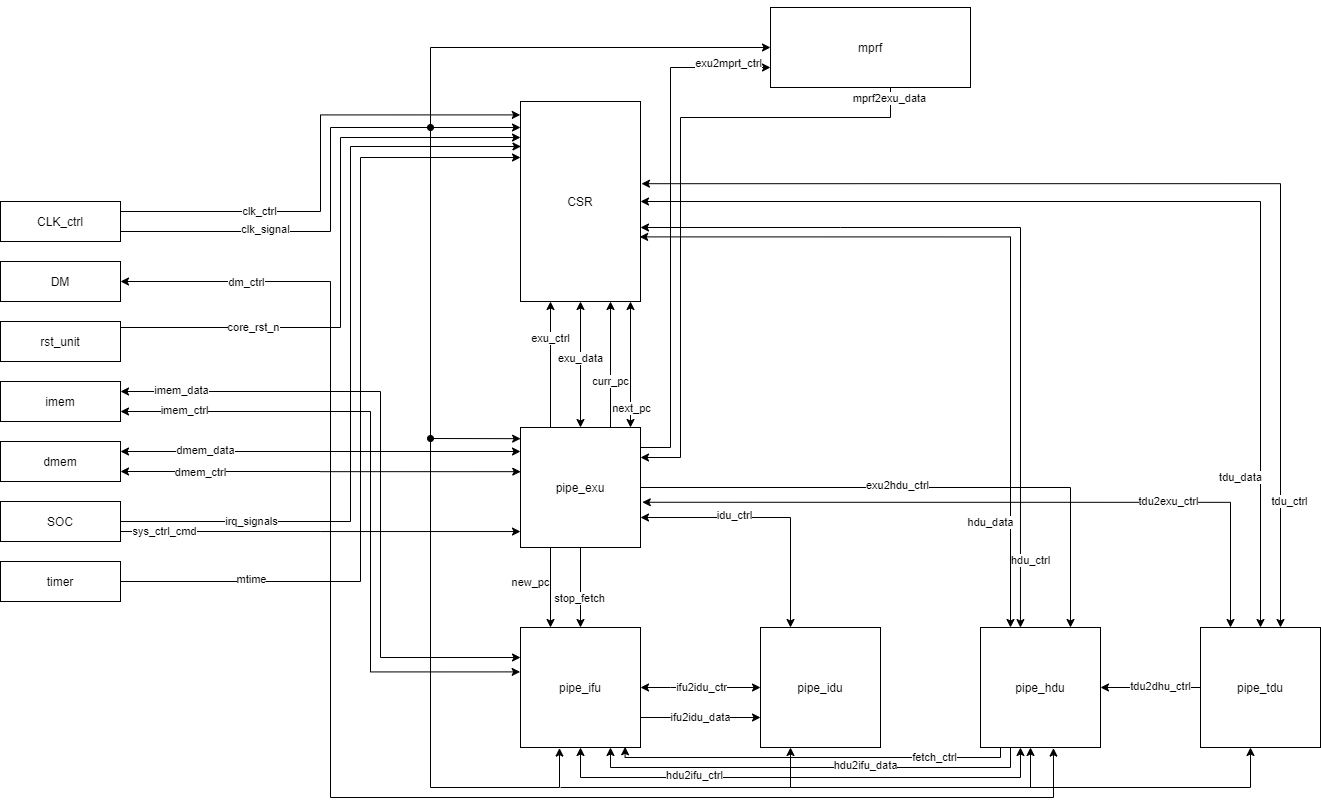
\includegraphics[width=\linewidth]{subfiles/imgs/pipetop.png}
    \caption{\centering Detailed reconstruction of block model}
    \label{scr1_blocks}
\end{figure}

Despite the completion of the internal signal definition, the complexity of the FMEA analysis procedure necessitated the use of the layout shown in Fig. \ref{classic_FMEA} as a worksheet. This layout served as a guide for the FMEA analysis team, who were tasked with identifying potential failures within the system and assessing the severity of their impact. However, the complexity of the system, as evidenced by the intricate interconnections between sub-blocks, proved to be a significant obstacle for the team, and the procedure was ultimately halted due to its difficulty. 

\begin{figure}[H]
    \centering
    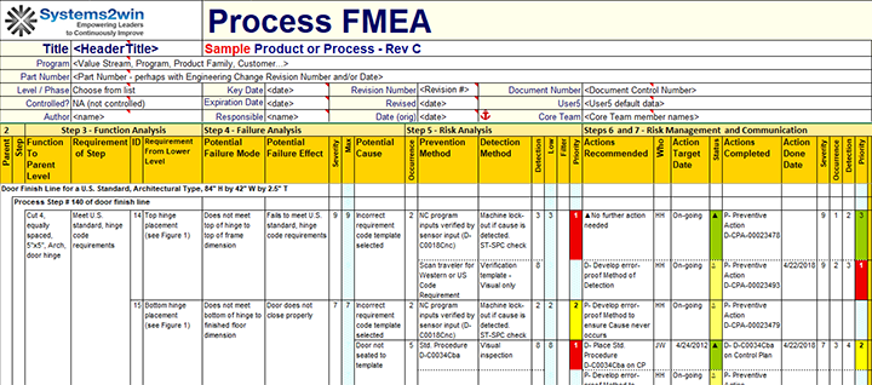
\includegraphics[width=\linewidth]{subfiles/imgs/old_fmea1.jpg.png}
    \caption{\centering Classic FMEA Worksheet layout}
    \label{classic_FMEA}
\end{figure}
Even with the aid of the layout, the team found that the manual identification of potential failures was too error-prone and time-consuming, necessitating a re-evaluation of the FMEA analysis process. A first detailed analysis of the possible failure modes and their gravity has been completed, and one extract can be seen in the Fig.\ref{classic_FMEA_SCR1} Despite this setback, the layout shown in Fig. \ref{scr1_blocks} remains a valuable tool for visualizing the internal workings of the core and can aid in future system design and analysis efforts.
\begin{figure}[H]
    \centering
    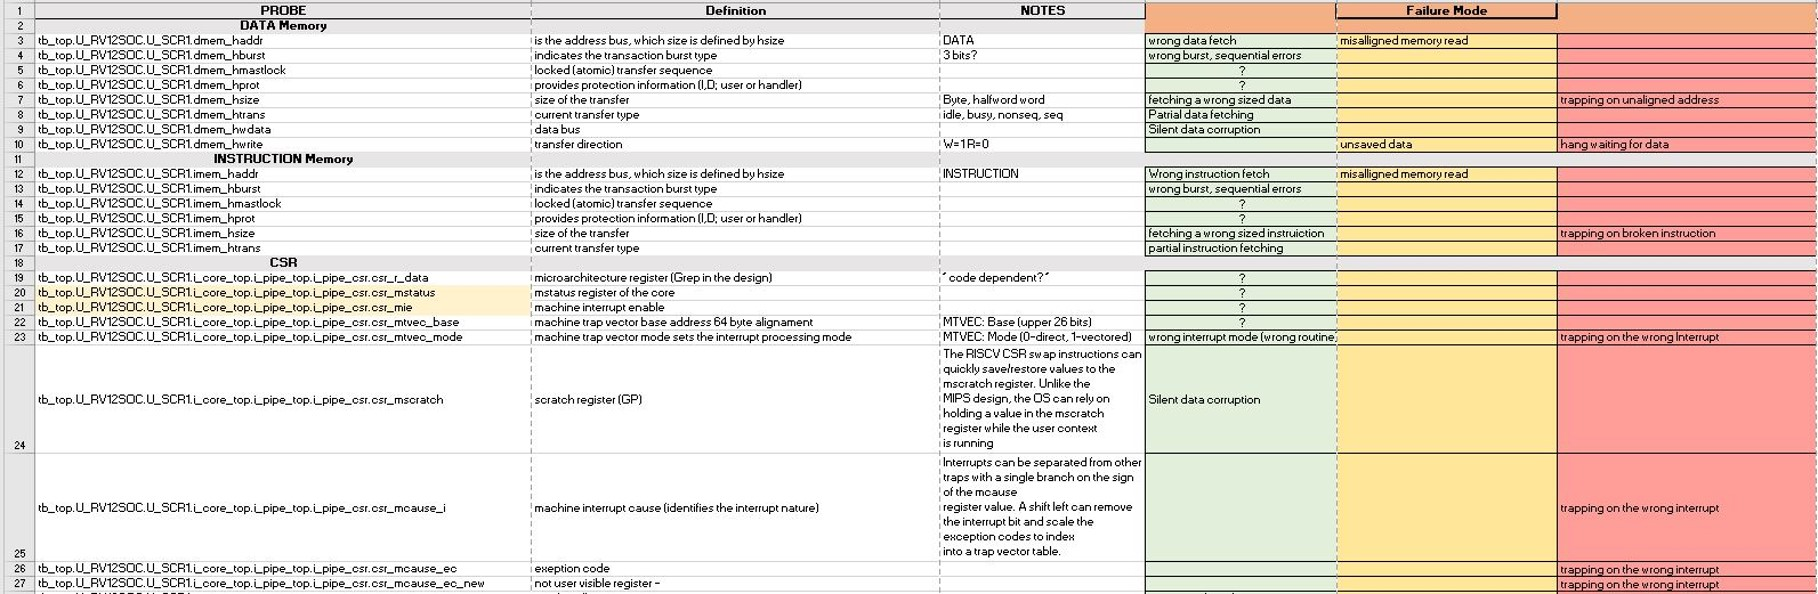
\includegraphics[angle=90, scale=0.6]{subfiles/imgs/old_fmea.jpg}
    \caption{\centering Classic FMEA Worksheet of SCR1}
    \label{classic_FMEA_SCR1}
\end{figure}

The difficulty encountered during the FMEA analysis procedure highlights the need to re-think the overall approach to system design and analysis. While the layout shown in Fig. \ref{scr1_blocks} provides a useful tool for visualizing system interconnections, it also underscores the need for more automated and efficient methods of identifying potential failures. By relying on manual analysis, the FMEA procedure is susceptible to human error and can be prohibitively time-consuming for complex systems like the one depicted in the figure. Moving forward, it may be necessary to explore more sophisticated analysis methods, such as automated approaches, to ensure that potential failures are identified and addressed in a timely and accurate manner.

\section{Modeling Digital Systems for MBSA}
\label{sec:modelling}
Digital systems, by essence, lend themselves well to finite state machines representation making the use of languages and formalism such as Altarica very suitable for their modelling. However, dysfunctional modeling requires extracting the faulty behaviour of the blocks composing the system. Such task is usually carried out by a Failure Mode and Effect Analysis (FMEA) to identify possible malfunction of the individual blocks. In digital system, such task can be performed automatically by simulation with fault injection\cite{6850649} and possibly formal methods \cite{7333399}.

The main issue in modelling digital systems for MBSA is choosing the adequate level of abstraction avoiding a direct $1 \Leftrightarrow 1$ translation of {\it Hardware Description Languages} (HDL) modeling concepts into Altarica. When extracting a safety model from a digital block three points must be addressed:
\begin{itemize}
    \item Structural hierarchy: Because Altarica support hierarchy \cite{PR14a}, translating hierarchy with adequate granularity can be straightforward, especially as natural design hierarchy is usually a good candidate.
    \item Behavioral modelling: Faulty behavioral aspects requires extraction of failure modes which can be performed manually, based on design knowledge or automatically using fault injection or formal approaches. Fault injection is well suited to such analysis, especially in the world of digital design which rely heavily on HDL simulators and digital fault injection driven by ISO26262 requirements. In this work we will exclusively focus on fault injection.
    \item Faults propagation: Blocks in a SoCs are usually connected though buses with well defined protocols and their failures modes ({\it unaligned access} \ldots) are known. The issue comes in the granularity of the modelling that, if too low will lead to too numerous events (1 HDL signal $\rightarrow$ 1 flow variable) while a too high abstraction may prevent catching of some protocol failures.
\end{itemize}
Fault injection campaigns are used to characterize the behavior of the system from its output pins point of view which are the 'vectors' for faults propagation between blocks. Also, knowing the functionality of each of these pins, it is possible to attach some possible consequences to the failure to such (group of) output(s). Such semantic labelling is, however, still manual and based on safety engineers knowledge and experience.


\section{Methodology}
\label{sec:methodology}
%it is possible to build an {\it extended} state 
On top of any explicit finite state machine or control code encoding the user specified behaviour, a more complete state exist that includes the totality of the signals belonging to the control path of a design, such as data states implicitly exposed in controls states, or implicitly coded control states. These signals compose a more complete and larger state machine exposing new states and transitions that are implicitly specified, for example resulting from Cartesian product of automatons. Those are, technically, the signals driving transitions conditions.

Combinations of these signals in those states can lead to a subtle set of fault states, difficult to identify from the HDL description as the encoding in this state machine is sparse due to correlations. Such argument comes from the fact that even for a small ($>\approx$50) number of flip-flops, the complete state space ($2^{50}$) cannot be traversed in a reasonable time. Therefore a non-negligible proportion of these states are what we call {\it illegal states} i.e. unreachable under normal behaviour, potentially leading to undesired and unspecified behavior when the block is exposed to those states though faults.

In order to build a failure model from a nominal behavioral {\it Register Transfer Model} (RTL) in Verilog or VHDL, behaviour of the system under faults must be analyzed and faulty behavior as well as failure modes must be extracted. We proceed using the following steps:
\begin{enumerate}
    \item {\it Identification and Extraction of State Signals}: Starting from the functional description, the set of flip-flops, belonging to both the {\it control} and possibly {\it data}) paths composing what we name as the {\it state}, has to be identified and extracted. This set, composed by all the flip-flops composing the control path and possibly the datapath which maintain the control state of the block, correspond to possible fault injection sites.
    %In digital systems, this state is composed by all the flip-flops composing the control path and possibly the datapath in some cases. 
    % of the control path
    %correspond to both the {\it control} and possibly {\it data}) state of the system and 
    %, as described in Fig.\ref{fig:prob_place}. 
    %\begin{figure}
    \centering



\tikzset{every picture/.style={line width=0.75pt}} %set default line width to 0.75pt        

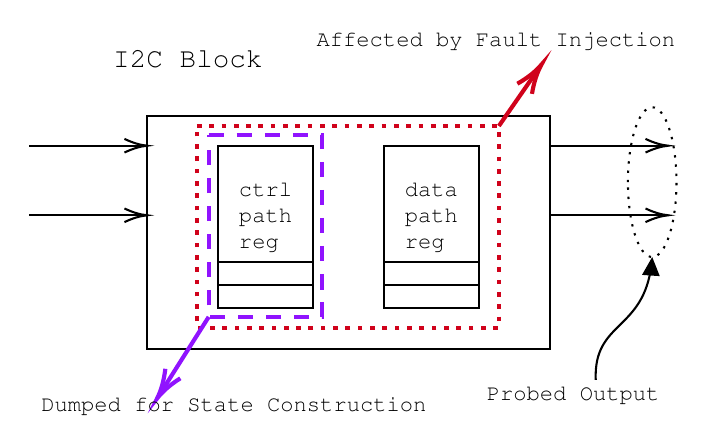
\begin{tikzpicture}[x=0.75pt,y=0.75pt,yscale=-1,xscale=1]
%uncomment if require: \path (0,300); %set diagram left start at 0, and has height of 300

%Shape: Rectangle [id:dp9326819923068139] 
\draw   (397.96,61.38) -- (591.95,61.38) -- (591.95,174) -- (397.96,174) -- cycle ;
%Straight Lines [id:da8579060622058785] 
\draw    (591.95,75.9) -- (647.01,75.9) ;
\draw [shift={(649.01,75.9)}, rotate = 180] [color={rgb, 255:red, 0; green, 0; blue, 0 }  ][line width=0.75]    (10.93,-3.29) .. controls (6.95,-1.4) and (3.31,-0.3) .. (0,0) .. controls (3.31,0.3) and (6.95,1.4) .. (10.93,3.29)   ;
%Straight Lines [id:da837066861655545] 
\draw    (591.95,109.42) -- (647.01,109.42) ;
\draw [shift={(649.01,109.42)}, rotate = 180] [color={rgb, 255:red, 0; green, 0; blue, 0 }  ][line width=0.75]    (10.93,-3.29) .. controls (6.95,-1.4) and (3.31,-0.3) .. (0,0) .. controls (3.31,0.3) and (6.95,1.4) .. (10.93,3.29)   ;
%Straight Lines [id:da0024830437913780923] 
\draw    (395.96,109.42) -- (340.91,109.42) ;
\draw [shift={(397.96,109.42)}, rotate = 180] [color={rgb, 255:red, 0; green, 0; blue, 0 }  ][line width=0.75]    (10.93,-3.29) .. controls (6.95,-1.4) and (3.31,-0.3) .. (0,0) .. controls (3.31,0.3) and (6.95,1.4) .. (10.93,3.29)   ;
%Straight Lines [id:da9595725272918905] 
\draw    (395.96,75.9) -- (367.15,75.9) -- (340.91,75.9) ;
\draw [shift={(397.96,75.9)}, rotate = 180] [color={rgb, 255:red, 0; green, 0; blue, 0 }  ][line width=0.75]    (10.93,-3.29) .. controls (6.95,-1.4) and (3.31,-0.3) .. (0,0) .. controls (3.31,0.3) and (6.95,1.4) .. (10.93,3.29)   ;
%Shape: Rectangle [id:dp3692381690862372] 
\draw   (432.2,75.9) -- (477.84,75.9) -- (477.84,154.11) -- (432.2,154.11) -- cycle ;
%Straight Lines [id:da641212380280751] 
\draw    (432.2,131.77) -- (477.84,131.77) ;
%Straight Lines [id:da016965396748415795] 
\draw    (432.2,142.94) -- (477.84,142.94) ;
%Shape: Rectangle [id:dp6397259288159378] 
\draw   (512.07,75.9) -- (557.72,75.9) -- (557.72,154.11) -- (512.07,154.11) -- cycle ;
%Straight Lines [id:da6619404417007224] 
\draw    (512.07,131.77) -- (557.72,131.77) ;
%Straight Lines [id:da5681218634155383] 
\draw    (512.07,142.94) -- (521.43,142.94) -- (557.72,142.94) ;
%Shape: Rectangle [id:dp700600527249986] 
\draw  [color={rgb, 255:red, 144; green, 19; blue, 254 }  ,draw opacity=1 ][dash pattern={on 5.63pt off 4.5pt}][line width=1.5]  (427.63,70.88) -- (482.4,70.88) -- (482.4,158.36) -- (427.63,158.36) -- cycle ;
%Shape: Rectangle [id:dp07083741234570073] 
\draw  [color={rgb, 255:red, 208; green, 2; blue, 27 }  ,draw opacity=1 ][dash pattern={on 1.69pt off 2.76pt}][line width=1.5]  (421.93,66.41) -- (567.42,66.41) -- (567.42,163.72) -- (421.93,163.72) -- cycle ;
%Straight Lines [id:da7847041731451427] 
\draw [color={rgb, 255:red, 144; green, 19; blue, 254 }  ,draw opacity=1 ][line width=1.5]    (427.63,158.36) -- (404.36,195.15) ;
\draw [shift={(402.75,197.68)}, rotate = 302.32] [color={rgb, 255:red, 144; green, 19; blue, 254 }  ,draw opacity=1 ][line width=1.5]    (14.21,-4.28) .. controls (9.04,-1.82) and (4.3,-0.39) .. (0,0) .. controls (4.3,0.39) and (9.04,1.82) .. (14.21,4.28)   ;
%Straight Lines [id:da28616250433266277] 
\draw [color={rgb, 255:red, 208; green, 2; blue, 27 }  ,draw opacity=1 ][line width=1.5]    (567.42,66.41) -- (586.25,39.27) ;
\draw [shift={(587.96,36.8)}, rotate = 484.75] [color={rgb, 255:red, 208; green, 2; blue, 27 }  ,draw opacity=1 ][line width=1.5]    (14.21,-4.28) .. controls (9.04,-1.82) and (4.3,-0.39) .. (0,0) .. controls (4.3,0.39) and (9.04,1.82) .. (14.21,4.28)   ;
%Shape: Ellipse [id:dp4541297034055598] 
\draw  [dash pattern={on 0.84pt off 2.51pt}] (629.61,93.44) .. controls (629.61,73.51) and (634.84,57.36) .. (641.3,57.36) .. controls (647.76,57.36) and (653,73.51) .. (653,93.44) .. controls (653,113.37) and (647.76,129.53) .. (641.3,129.53) .. controls (634.84,129.53) and (629.61,113.37) .. (629.61,93.44) -- cycle ;
%Curve Lines [id:da48121849953597806] 
\draw    (641.01,132.69) .. controls (637.21,165.58) and (612.98,160.03) .. (614.09,188.74) ;
\draw [shift={(641.3,129.53)}, rotate = 94.03] [fill={rgb, 255:red, 0; green, 0; blue, 0 }  ][line width=0.08]  [draw opacity=0] (8.93,-4.29) -- (0,0) -- (8.93,4.29) -- cycle    ;

% Text Node
\draw (455.02,128.66) node [anchor=south] [inner sep=0.75pt]  [font=\footnotesize] [align=left] {{\fontfamily{pcr}\selectfont ctrl}\\{\fontfamily{pcr}\selectfont path}\\{\fontfamily{pcr}\selectfont reg}};
% Text Node
\draw (534.9,128.66) node [anchor=south] [inner sep=0.75pt]  [font=\footnotesize] [align=left] {{\fontfamily{pcr}\selectfont data}\\{\fontfamily{pcr}\selectfont path}\\{\fontfamily{pcr}\selectfont reg}};
% Text Node
\draw (380.14,28.21) node [anchor=north west][inner sep=0.75pt]   [align=left] {{\fontfamily{pcr}\selectfont I2C Block}};
% Text Node
\draw (345.47,195.16) node [anchor=north west][inner sep=0.75pt]  [font=\footnotesize] [align=left] {{\footnotesize {\fontfamily{pcr}\selectfont Dumped for State Construction}}};
% Text Node
\draw (478.09,19.53) node [anchor=north west][inner sep=0.75pt]  [font=\footnotesize] [align=left] {{\footnotesize {\fontfamily{pcr}\selectfont Affected by Fault Injection}}};
% Text Node
\draw (560.12,190.47) node [anchor=north west][inner sep=0.75pt]  [font=\footnotesize] [align=left] {{\footnotesize {\fontfamily{pcr}\selectfont Probed Output}}};


\end{tikzpicture}
    \caption{scheme of probes placement and affected/dumped registers}
    \label{fig:prob_place}
\end{figure} 

    \item {\it Testbench Setup} : A standalone testbench is set up with care given to coverage and testbench representability as the states traversed during this golden execution will serve as non-faulty reference behavior. Tools like \textit{Incisive Metrics Coverage} (IMC) \cite{CDN} or \textit{Certitude} \cite{Certitude} can be used to assess testbench coverage. A first reference run is performed to allow extraction of golden functional states that will be used later in the process to be differentiated from non-functional ones under fault injection.
    
    \item {\it Fault Injection Campaign}: Fault injection is the mean by which the misbehavior and faulty execution is exposed on purposes. Probes (i.e., observation points) are defined during the setup of the fault injection campaign. They are set on the outputs of all blocks in order to identify failures that propagates to other blocks. Probes monitor and compare the probed signal value at each clock cycle with the golden reference and report any difference. They have been set to stop simulation when a fault reaches an output of the design. This step is the core of our analysis aimed at extracting faulty behaviour, modes and effects though exploration of the faulty states by fault injection.

    \item {\it Extraction of Faulty Behavior}: Once the faulty runs have completed, non-functional (i.e. {\it faulty}) states and behavior are extracted by subtracting functional ({\it golden}) states taken from the golden run state dictionary to the faulty run states, leaving only newly discovered faulty states and transitions.

    \item {\it Construction of the Faulty Model}: The newly discovered states and transitions are used to augment the functional models with faulty behavior. Transitions from a functional to a non-functional state are labeled with the responsible faults so are states responsible for an incorrect output. This model serves as a base for the translation into the Altarica language.
\end{enumerate}
Currently, the method is limited in the {\it effect} analysis of the FMEA. Effect such as {\it loss of power} cannot be attached automatically to a faulty state as it would requires an inference and abstraction process out the reach of the tool currently. Thus, such labelling is performed manually by attaching effects to outputs and then back-propagating them into the states and faults responsible for the given outputs corruptions.

\subsection{Faulty Behavior Model Construction}
\label{FBMC}
Once the faulty behavior has been extracted from faulty runs, the faulty model can be constructed using graph analysis algorithms. The first step in the model construction is collapsing states that are not meaningful for the dysfunctional model. We proceed currently with the following rules:
\begin{itemize}
    \item Any component (connected subgraph) comprising only legal states and legal transitions are collapsed into one single {\it functional} state.
    \item Legal states with illegal transitions or incorrect outputs (outputs values do differs from reference in these states) are kept and illegal transition probabilities are attached.
    \item Any component comprising only nodes not propagating any faults to outputs are collapsed into one single {\it faulty} state. Probabilities to enter this state can be extracted from transitions leading to the collapsed states.
    \item Faulty nodes propagating faults to outputs are kept and transitions probabilities are attached to allow computing incorrect outputs probabilities.
    \item Effect attached to output pins are back propagated in the state graph faulty states where output corruptions occurs.
\end{itemize}
However additional rules may be added like to remove faulty nodes and transitions from masked faults for example, especially those not leading to any latent faults (execution is correct with no faults propagated to outputs and internal state doesn't differs from reference one at some point, i.e. fault has {\it vanished}). We ultimately target discrete-time Markov chains \cite{lec3_dtmc_p1} for our dysfunctional behaviour modelling (Fig. \ref{altarica-model}).


%
\begin{figure}[h]
\centering
\tikzset{every picture/.style={line width=0.75pt}} %set default line width to 0.75pt        

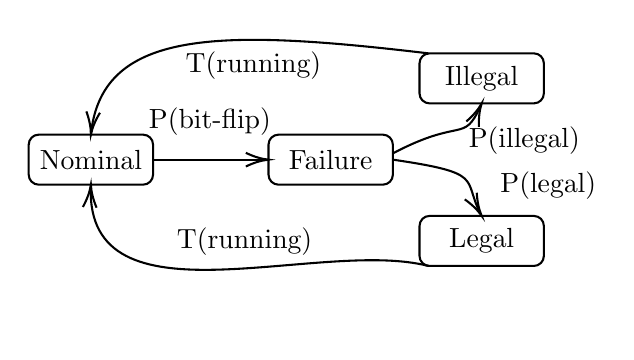
\begin{tikzpicture}[x=0.75pt,y=0.75pt,yscale=-1,xscale=1]
%uncomment if require: \path (0,235); %set diagram left start at 0, and has height of 235

%Rounded Rect [id:dp4097096976762369] 
\draw   (10,64.69) .. controls (10,62.02) and (12.16,59.87) .. (14.82,59.87) -- (65.09,59.87) .. controls (67.75,59.87) and (69.91,62.02) .. (69.91,64.69) -- (69.91,79.15) .. controls (69.91,81.81) and (67.75,83.97) .. (65.09,83.97) -- (14.82,83.97) .. controls (12.16,83.97) and (10,81.81) .. (10,79.15) -- cycle ;
%Rounded Rect [id:dp2835435765541303] 
\draw   (125.54,64.69) .. controls (125.54,62.02) and (127.7,59.87) .. (130.36,59.87) -- (180.63,59.87) .. controls (183.29,59.87) and (185.45,62.02) .. (185.45,64.69) -- (185.45,79.15) .. controls (185.45,81.81) and (183.29,83.97) .. (180.63,83.97) -- (130.36,83.97) .. controls (127.7,83.97) and (125.54,81.81) .. (125.54,79.15) -- cycle ;
%Rounded Rect [id:dp5805736774223651] 
\draw   (198.29,25.52) .. controls (198.29,22.86) and (200.45,20.7) .. (203.11,20.7) -- (253.38,20.7) .. controls (256.04,20.7) and (258.2,22.86) .. (258.2,25.52) -- (258.2,39.98) .. controls (258.2,42.64) and (256.04,44.8) .. (253.38,44.8) -- (203.11,44.8) .. controls (200.45,44.8) and (198.29,42.64) .. (198.29,39.98) -- cycle ;
%Rounded Rect [id:dp8614575685420135] 
\draw   (198.29,103.85) .. controls (198.29,101.19) and (200.45,99.03) .. (203.11,99.03) -- (253.38,99.03) .. controls (256.04,99.03) and (258.2,101.19) .. (258.2,103.85) -- (258.2,118.31) .. controls (258.2,120.97) and (256.04,123.13) .. (253.38,123.13) -- (203.11,123.13) .. controls (200.45,123.13) and (198.29,120.97) .. (198.29,118.31) -- cycle ;
%Curve Lines [id:da16079762072366677] 
\draw    (185.45,68.9) .. controls (218.66,51.37) and (219.45,64.08) .. (227.48,46.52) ;
\draw [shift={(228.25,44.8)}, rotate = 113.59] [color={rgb, 255:red, 0; green, 0; blue, 0 }  ][line width=0.75]    (10.93,-3.29) .. controls (6.95,-1.4) and (3.31,-0.3) .. (0,0) .. controls (3.31,0.3) and (6.95,1.4) .. (10.93,3.29)   ;
%Curve Lines [id:da04663923009445026] 
\draw    (185.45,71.92) .. controls (229.87,78.4) and (219.12,81.01) .. (227.42,97.46) ;
\draw [shift={(228.25,99.03)}, rotate = 241.15] [color={rgb, 255:red, 0; green, 0; blue, 0 }  ][line width=0.75]    (10.93,-3.29) .. controls (6.95,-1.4) and (3.31,-0.3) .. (0,0) .. controls (3.31,0.3) and (6.95,1.4) .. (10.93,3.29)   ;
%Straight Lines [id:da44802200900780054] 
\draw    (69.91,71.92) -- (123.54,71.92) ;
\draw [shift={(125.54,71.92)}, rotate = 180] [color={rgb, 255:red, 0; green, 0; blue, 0 }  ][line width=0.75]    (10.93,-3.29) .. controls (6.95,-1.4) and (3.31,-0.3) .. (0,0) .. controls (3.31,0.3) and (6.95,1.4) .. (10.93,3.29)   ;
%Curve Lines [id:da03387373961296125] 
\draw    (202.57,20.7) .. controls (102.59,8.83) and (46.22,8.86) .. (40.12,58.35) ;
\draw [shift={(39.96,59.87)}, rotate = 275.75] [color={rgb, 255:red, 0; green, 0; blue, 0 }  ][line width=0.75]    (10.93,-3.29) .. controls (6.95,-1.4) and (3.31,-0.3) .. (0,0) .. controls (3.31,0.3) and (6.95,1.4) .. (10.93,3.29)   ;
%Curve Lines [id:da005071296130858216] 
\draw    (202.57,123.13) .. controls (149.77,109.55) and (37.45,154.22) .. (39.91,85.02) ;
\draw [shift={(39.96,83.97)}, rotate = 92.95] [color={rgb, 255:red, 0; green, 0; blue, 0 }  ][line width=0.75]    (10.93,-3.29) .. controls (6.95,-1.4) and (3.31,-0.3) .. (0,0) .. controls (3.31,0.3) and (6.95,1.4) .. (10.93,3.29)   ;

% Text Node
\draw (39.96,71.92) node   [align=left] {Nominal};
% Text Node
\draw (155.5,71.92) node   [align=left] {Failure};
% Text Node
\draw (228.25,32.75) node   [align=left] {Illegal};
% Text Node
\draw (228.25,111.08) node   [align=left] {Legal};
% Text Node
\draw (248.79,62.58) node   [align=left] {P(illegal)};
% Text Node
\draw (260.34,84.27) node   [align=left] {P(legal)};
% Text Node
\draw (118.27,26.43) node   [align=left] {T(running)};
% Text Node
\draw (113.99,111.38) node   [align=left] {T(running)};
% Text Node
\draw (97.3,53.54) node   [align=left] {P(bit-flip)};

\end{tikzpicture}
\caption{Altarica Dysfunctional Model}
\label{altarica-model}
\end{figure}

\begin{figure}[!ht]
    \centering
    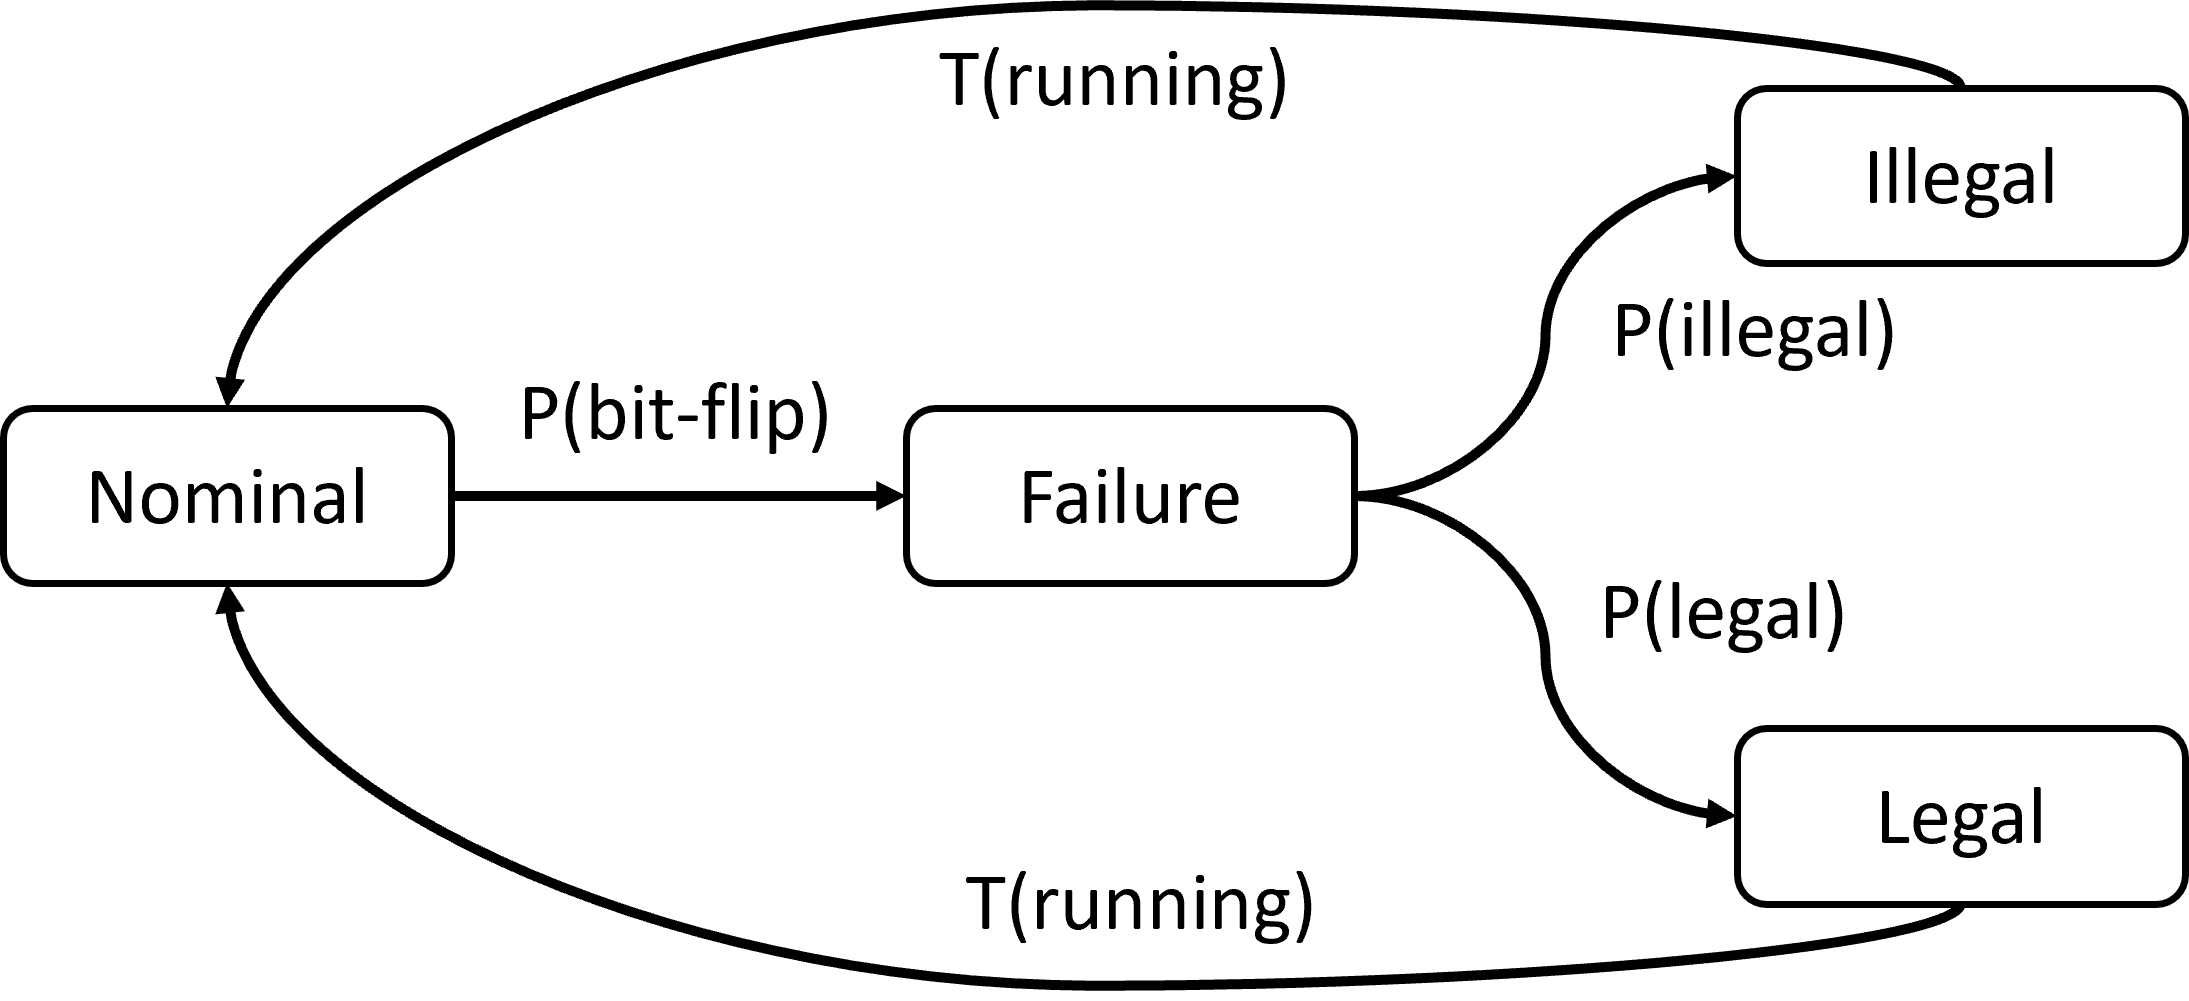
\includegraphics[width=\linewidth]{subfiles/imgs/altarica-dysfunctional-model.png}
    \caption{\centering Altarica Dysfunctional Model}
    \label{altarica-model}
\end{figure}

\subsection{Completeness of Extraction}
The main risk in state identification is to under or overestimate the state which would lead to uncovered faulty states (fault not injected in a flip-flop misidentified as not {\it control}) or over estimate the state leading to classification of what are, in fact, data state as control states. The latter can be easily identified as randomizing data in the golden or faulty state machine extraction step leads to an increasing number of states with the number of runs. On Fig. \ref{fig:completness-extraction}, a correct identification leads to a saturating number of states (green curves) while an incorrect one leads to a diverging number of states as the number of tests grows (red curve).

\begin{figure}[!ht]
    \centering
    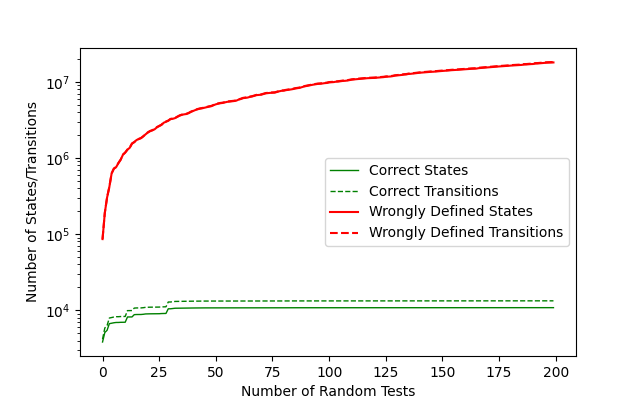
\includegraphics[width=\linewidth]{subfiles/imgs/wrongly_identified_for_paper.png}
    \caption{\centering Completeness of the Extraction}
    \label{fig:completness-extraction}
\end{figure}


%We verify that standalone extraction of the faulty model is complete, that is no new faulty behavior appear when the DUT is integrated and studied in the complete system. Thus the same stages as depicted in section \ref{sec:methodology} are performed on the complete system composed of the I2C+AHB system.

\subsection{Altarica Modeling}
\label{sec:results}
%Data gathered by the application of the methodology is then elaborated starting from data shown in table and the dictionaries collecting all states and transitions, created at faulty behavior extraction phase. 

Such an automaton representation is adequate for Altarica modelling as described below. When performing translation to Altarica, two elements shall be extracted:
\begin{enumerate}
    \item The internal state machine corresponding to failures.
    \item The assertion part corresponding to the propagation failure probability from input to one or more output of element.
\end{enumerate}
Base modelling must include at least four states (Fig. \ref{fig:simp_fsm}): a {\it nominal} state where no failure occurs, a {\it failure} state corresponding to a bit-flip error injection and an {\it illegal} state corresponding to propagation of the failure to one or more outputs. The {\it legal} state correspond to failures leading to legals transitions, without failure propagation to outputs.

 Assertions on outputs are conditioned by the internal state machine and inputs of the block. Every time internal state machine is in the illegal state, outputs values are updated. In same way, if one input of the block is set in the failed state, outputs are updated. Probabilities to generate a faulty output or to propagate failures from inputs to outputs are extracted from fault injection campaigns (Table \ref{block_full_system_fi_results}). Currently, all illegal states are collapsed into a single one, but different non-functional states corresponding to different failure modes can be extracted as well, such as represented on Fig. \ref{fig:simp_fsm} where two illegal states are identified whether or not a simulation timeout (10\% of golden execution time) occurs. Criteria for refined dysfunctional automaton extraction are not yet addressed as well as construction and reduction rules from fault injection data for such an automaton.

%Internal state machine of each element shall be extracted based on fault campaign results. 
%The internal state machine correspond to behavior of element in case failure corresponding to a bit-flip. 

\section{Application: {\it I2C} to {\it AHB} bridge} \label{application}
In order to exercise the methodology presented in Section \ref{sec:methodology}, we use a test case composed of 2 blocks: an {\it I2C} slave \cite{mankar2014review} connected to an {\it AHB} \cite{9063856} bus master interface (Fig. \ref{fig:complete_system}). Commands ({\it read} or {\it write}) along with parameters ({\it address} and {\it data}) are received on the serial line and transformed into a series of AHB read and write transactions. Such a system, composed of two interconnected blocks, is humanely understandable so are its dysfunctional modes, while being complex enough to detail thoroughly the methodology.

The I2C slave, taken from \cite{I2Cminion}, receives {\it read} or {\it write} commands followed by an address byte and an optional data byte. On an I2C read, the byte returned from the AHB read transaction is returned. chronogramm for the read and write sequences are represented on Fig. \ref{fig:chronogluewrite}. The system is represented on Fig. \ref{fig:complete_system}. At both end of the system (I2C input and AHB output buses), I2C master and AHB slave Verification IPs (VIP) are attached to generate and verify correctness of I2C and AHB transactions.

\begin{figure}[h]
    \centering



\tikzset{every picture/.style={line width=0.75pt}} %set default line width to 0.75pt        

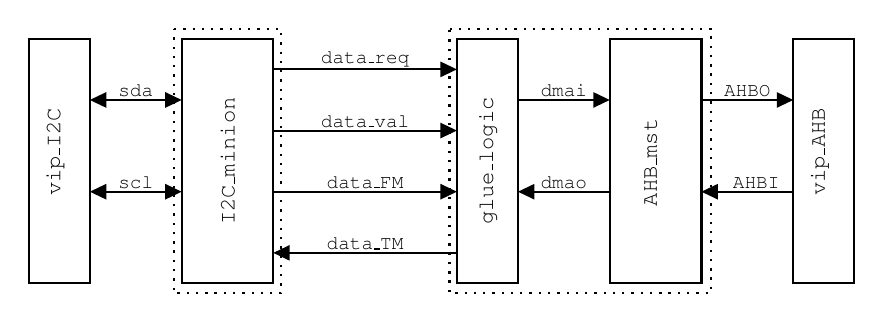
\begin{tikzpicture}[x=0.85pt,y=0.85pt,yscale=-1.3,xscale=1.3]
%uncomment if require: \path (0,300); %set diagram left start at 0, and has height of 300

%Shape: Rectangle [id:dp4079589054406878] 
\draw   (70,60) -- (100,60) -- (100,140) -- (70,140) -- cycle ;
%Shape: Rectangle [id:dp32174966169393304] 
\draw   (160,60) -- (180,60) -- (180,140) -- (160,140) -- cycle ;
%Shape: Rectangle [id:dp8708617087982464] 
\draw   (210,60) -- (240,60) -- (240,140) -- (210,140) -- cycle ;
%Shape: Rectangle [id:dp6411738601274033] 
\draw   (270,60) -- (290,60) -- (290,140) -- (270,140) -- cycle ;
%Shape: Rectangle [id:dp537675519060894] 
\draw   (20,60) -- (40,60) -- (40,140) -- (20,140) -- cycle ;
%Shape: Rectangle [id:dp738814812078364] 
\draw  [dash pattern={on 0.84pt off 2.51pt}] (67.5,56.75) -- (102.5,56.75) -- (102.5,143.25) -- (67.5,143.25) -- cycle ;
%Shape: Rectangle [id:dp16028896948499805] 
\draw  [dash pattern={on 0.84pt off 2.51pt}] (157.6,56.7) -- (243,56.7) -- (243,143.2) -- (157.6,143.2) -- cycle ;
%Straight Lines [id:da14064721488292253] 
\draw    (43,80) -- (67,80) ;
\draw [shift={(70,80)}, rotate = 180] [fill={rgb, 255:red, 0; green, 0; blue, 0 }  ][line width=0.08]  [draw opacity=0] (5.36,-2.57) -- (0,0) -- (5.36,2.57) -- cycle    ;
\draw [shift={(40,80)}, rotate = 0] [fill={rgb, 255:red, 0; green, 0; blue, 0 }  ][line width=0.08]  [draw opacity=0] (5.36,-2.57) -- (0,0) -- (5.36,2.57) -- cycle    ;
%Straight Lines [id:da4386174351987262] 
\draw    (43,110) -- (67,110) ;
\draw [shift={(70,110)}, rotate = 180] [fill={rgb, 255:red, 0; green, 0; blue, 0 }  ][line width=0.08]  [draw opacity=0] (5.36,-2.57) -- (0,0) -- (5.36,2.57) -- cycle    ;
\draw [shift={(40,110)}, rotate = 0] [fill={rgb, 255:red, 0; green, 0; blue, 0 }  ][line width=0.08]  [draw opacity=0] (5.36,-2.57) -- (0,0) -- (5.36,2.57) -- cycle    ;
%Straight Lines [id:da5336477753811442] 
\draw    (100,70) -- (157,70) ;
\draw [shift={(160,70)}, rotate = 180] [fill={rgb, 255:red, 0; green, 0; blue, 0 }  ][line width=0.08]  [draw opacity=0] (5.36,-2.57) -- (0,0) -- (5.36,2.57) -- cycle    ;
%Straight Lines [id:da5216454033214535] 
\draw    (100,90) -- (157,90) ;
\draw [shift={(160,90)}, rotate = 180] [fill={rgb, 255:red, 0; green, 0; blue, 0 }  ][line width=0.08]  [draw opacity=0] (5.36,-2.57) -- (0,0) -- (5.36,2.57) -- cycle    ;
%Straight Lines [id:da06972034582349096] 
\draw    (100,110) -- (157,110) ;
\draw [shift={(160,110)}, rotate = 180] [fill={rgb, 255:red, 0; green, 0; blue, 0 }  ][line width=0.08]  [draw opacity=0] (5.36,-2.57) -- (0,0) -- (5.36,2.57) -- cycle    ;
%Straight Lines [id:da16308212972517788] 
\draw    (103,130) -- (160,130) ;
\draw [shift={(100,130)}, rotate = 0] [fill={rgb, 255:red, 0; green, 0; blue, 0 }  ][line width=0.08]  [draw opacity=0] (5.36,-2.57) -- (0,0) -- (5.36,2.57) -- cycle    ;
%Straight Lines [id:da04498796035539643] 
\draw    (180,80) -- (207,80) ;
\draw [shift={(210,80)}, rotate = 180] [fill={rgb, 255:red, 0; green, 0; blue, 0 }  ][line width=0.08]  [draw opacity=0] (5.36,-2.57) -- (0,0) -- (5.36,2.57) -- cycle    ;
%Straight Lines [id:da9819499243578742] 
\draw    (183,110) -- (210,110) ;
\draw [shift={(180,110)}, rotate = 0] [fill={rgb, 255:red, 0; green, 0; blue, 0 }  ][line width=0.08]  [draw opacity=0] (5.36,-2.57) -- (0,0) -- (5.36,2.57) -- cycle    ;
%Straight Lines [id:da4892721330990073] 
\draw    (240,80) -- (267,80) ;
\draw [shift={(270,80)}, rotate = 180] [fill={rgb, 255:red, 0; green, 0; blue, 0 }  ][line width=0.08]  [draw opacity=0] (5.36,-2.57) -- (0,0) -- (5.36,2.57) -- cycle    ;
%Straight Lines [id:da9092580589886958] 
\draw    (243,110) -- (245.8,110) -- (270,110) ;
\draw [shift={(240,110)}, rotate = 0] [fill={rgb, 255:red, 0; green, 0; blue, 0 }  ][line width=0.08]  [draw opacity=0] (5.36,-2.57) -- (0,0) -- (5.36,2.57) -- cycle    ;

% Text Node
\draw (28.5,97) node  [font=\footnotesize,rotate=-270] [align=left] {{\fontfamily{pcr}\selectfont vip\_I2C}};
% Text Node
\draw (85,100) node  [font=\footnotesize,rotate=-270] [align=left] {{\fontfamily{pcr}\selectfont I2C\_minion}};
% Text Node
\draw (170,100) node  [font=\footnotesize,rotate=-270] [align=left] {{\fontfamily{pcr}\selectfont glue\_logic}};
% Text Node
\draw (223.4,100.4) node  [font=\footnotesize,rotate=-270] [align=left] {{\fontfamily{pcr}\selectfont AHB\_mst}};
% Text Node
\draw (278.5,97) node  [font=\footnotesize,rotate=-270] [align=left] {{\fontfamily{pcr}\selectfont vip\_AHB}};
% Text Node
\draw (55,80) node [anchor=south] [inner sep=0.75pt]  [font=\scriptsize] [align=left] {{\fontfamily{pcr}\selectfont sda}};
% Text Node
\draw (55,110) node [anchor=south] [inner sep=0.75pt]  [font=\scriptsize] [align=left] {{\fontfamily{pcr}\selectfont scl}};
% Text Node
\draw (130,70) node [anchor=south] [inner sep=0.75pt]  [font=\scriptsize] [align=left] {{\fontfamily{pcr}\selectfont data\_req}};
% Text Node
\draw (130,90) node [anchor=south] [inner sep=0.75pt]  [font=\scriptsize] [align=left] {{\fontfamily{pcr}\selectfont data\_val}};
% Text Node
\draw (130,110) node [anchor=south] [inner sep=0.75pt]  [font=\scriptsize] [align=left] {{\fontfamily{pcr}\selectfont data\_FM}};
% Text Node
\draw (130,130) node [anchor=south] [inner sep=0.75pt]  [font=\scriptsize] [align=left] {{\fontfamily{pcr}\selectfont data\_TM}};
% Text Node
\draw (195,80) node [anchor=south] [inner sep=0.75pt]  [font=\scriptsize] [align=left] {{\fontfamily{pcr}\selectfont dmai}};
% Text Node
\draw (195,110) node [anchor=south] [inner sep=0.75pt]  [font=\scriptsize] [align=left] {{\fontfamily{pcr}\selectfont dmao}};
% Text Node
\draw (255,80) node [anchor=south] [inner sep=0.75pt]  [font=\scriptsize] [align=left] {{\fontfamily{pcr}\selectfont AHBO}};
% Text Node
\draw (257.9,110) node [anchor=south] [inner sep=0.75pt]  [font=\scriptsize] [align=left] {{\fontfamily{pcr}\selectfont AHBI}};


\end{tikzpicture}
    \caption{I2C to AHB System Block Diagram}
    \label{fig:complete_system}
\end{figure}

\begin{figure}[!h]
    \centering
    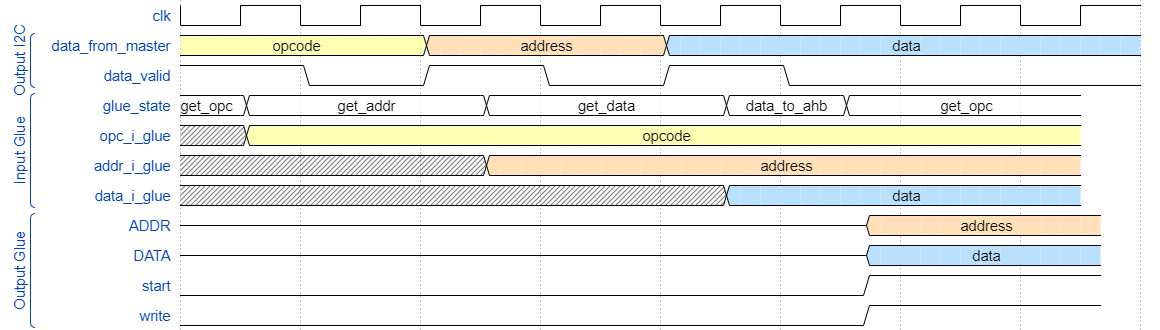
\includegraphics[width=\linewidth]{subfiles/imgs/chrono_write.png}
    \caption{I2C/AHB System Model}
    \label{fig:chronogluewrite}
\end{figure}

%\begin{table}[]
%\centering
%\caption{Coverage Figures for the I2C block}
%\begin{tabular}{|l|l|l|l|}
%\hline
%                    & Total & Covered & \textbf{\%} \\ \hline
%State Coverage      & 8     & 8       & 100         \\ \hline
%Transition Coverage & 25    & 13      & 53          \\ \hline
%\end{tabular}
%\label{tab:cov_I2C_modelsim}
%\end{table}

\subsection{I2C Block Modeling} \label{i2ctestcase}

The testbench is composed of a series of read and write random transactions. The coverage evaluation of the design has been carried out, results are presented in Table \ref{tab:cov_I2C}. Having considered the results of the coverage evaluations sufficient for the demonstration, application of the method presented in section \ref{sec:methodology} have been performed. The list of all injection sites, reported by Cadence {\it Xcelium Fault Simulator} (FSV) \cite{CDN} fault injection tool are considered for state including ones containing data as the serial nature of the I2C protocol, which mixes control and data frames on the same signals thought time-multiplexing, doesn't allow differentiation. However, the small size of data considered (8-bit) only induce a low (256) superset of the real control states. All outputs are probed so that any mismatch with the reference run will stop the simulation and report the fault as {\it Detected}. State (flip-flop value, i.e. '0' or '1') is simply extracted at each clock cycle and printed in the simulation logs to be post-processed.

\begin{figure}
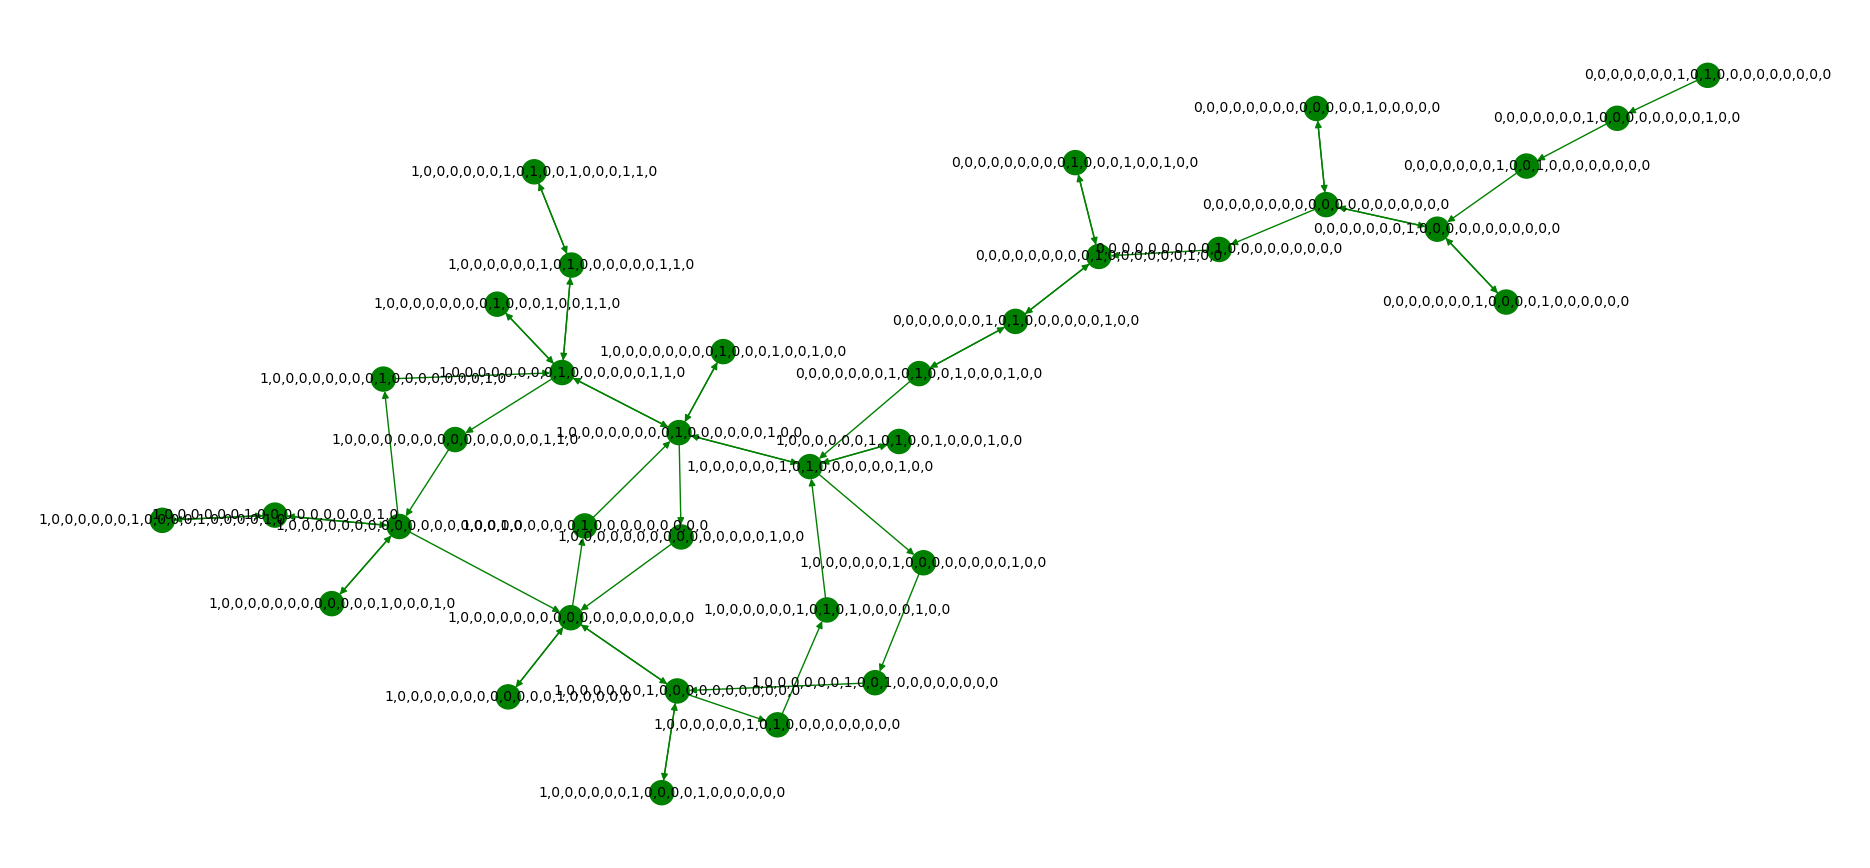
\includegraphics[width=\linewidth]{subfiles/imgs/I2C_gold_automaton_10.png}
\caption{I2C Gold Automaton}
\label{fig:I2C_gold}


\end{figure}

\begin{figure}
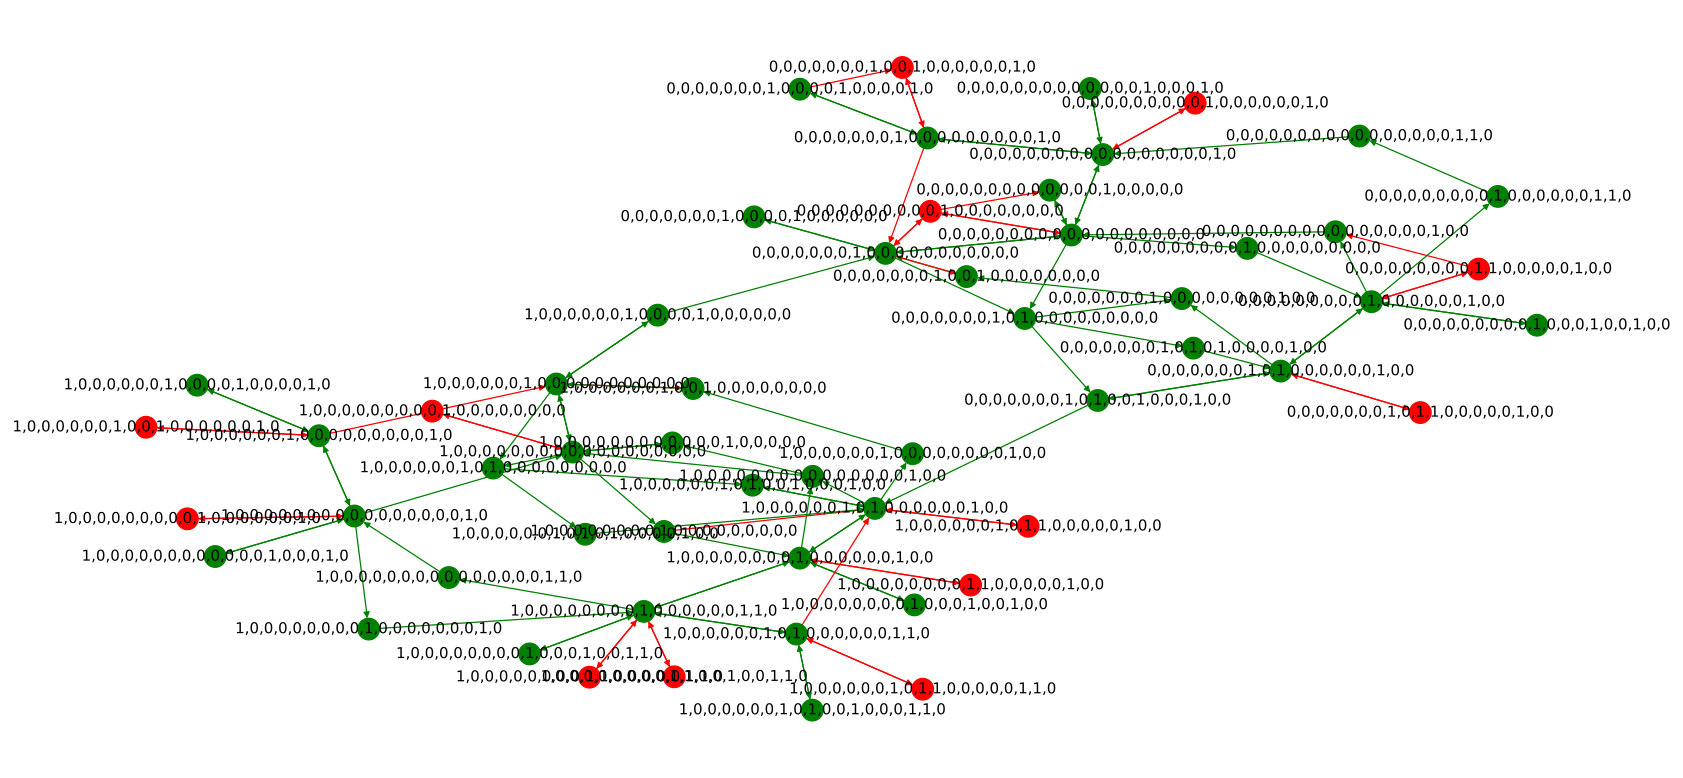
\includegraphics[width=\linewidth]{subfiles/imgs/I2C_complete_automaton_10.png}
\caption{I2C Complete Automaton}
\label{fig:I2C_goldcomplete}
\end{figure}

\begin{figure}
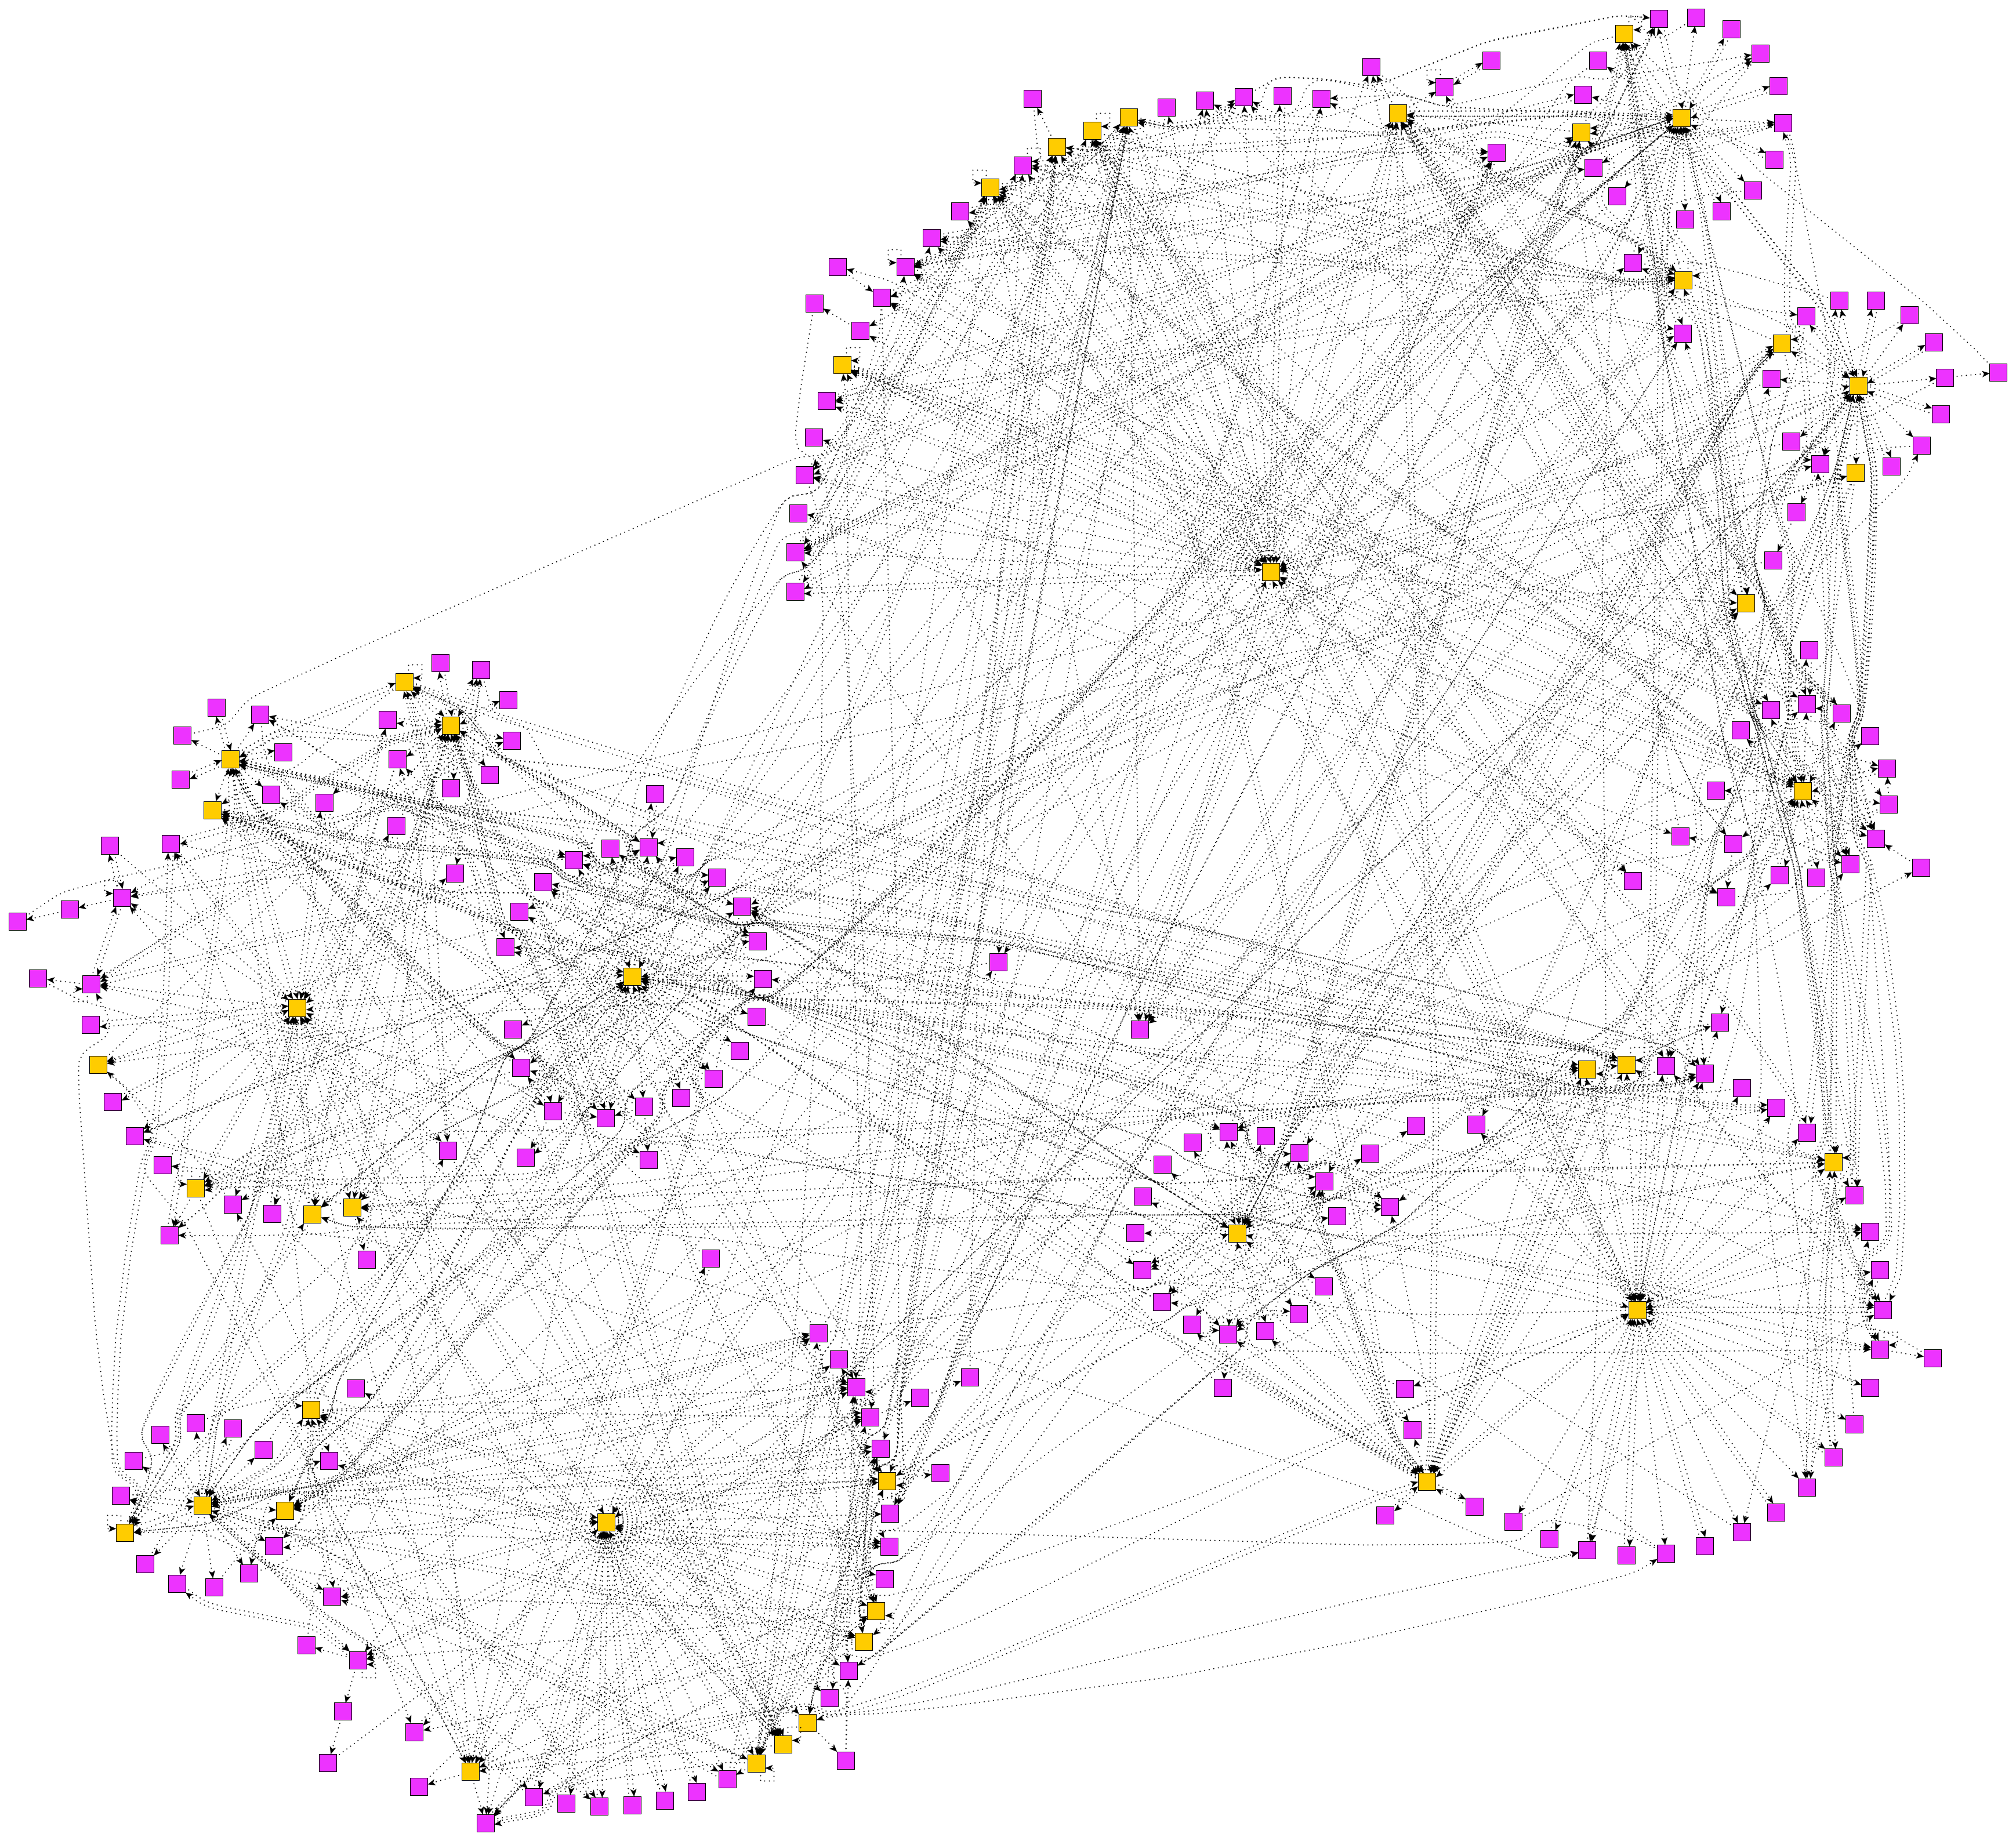
\includegraphics[width=\linewidth]{subfiles/imgs/i2c_balloon_injec.png}
\caption{I2C Complete Automaton Clusterized}
\label{fig:I2C_balloon}
\end{figure}

\begin{figure}
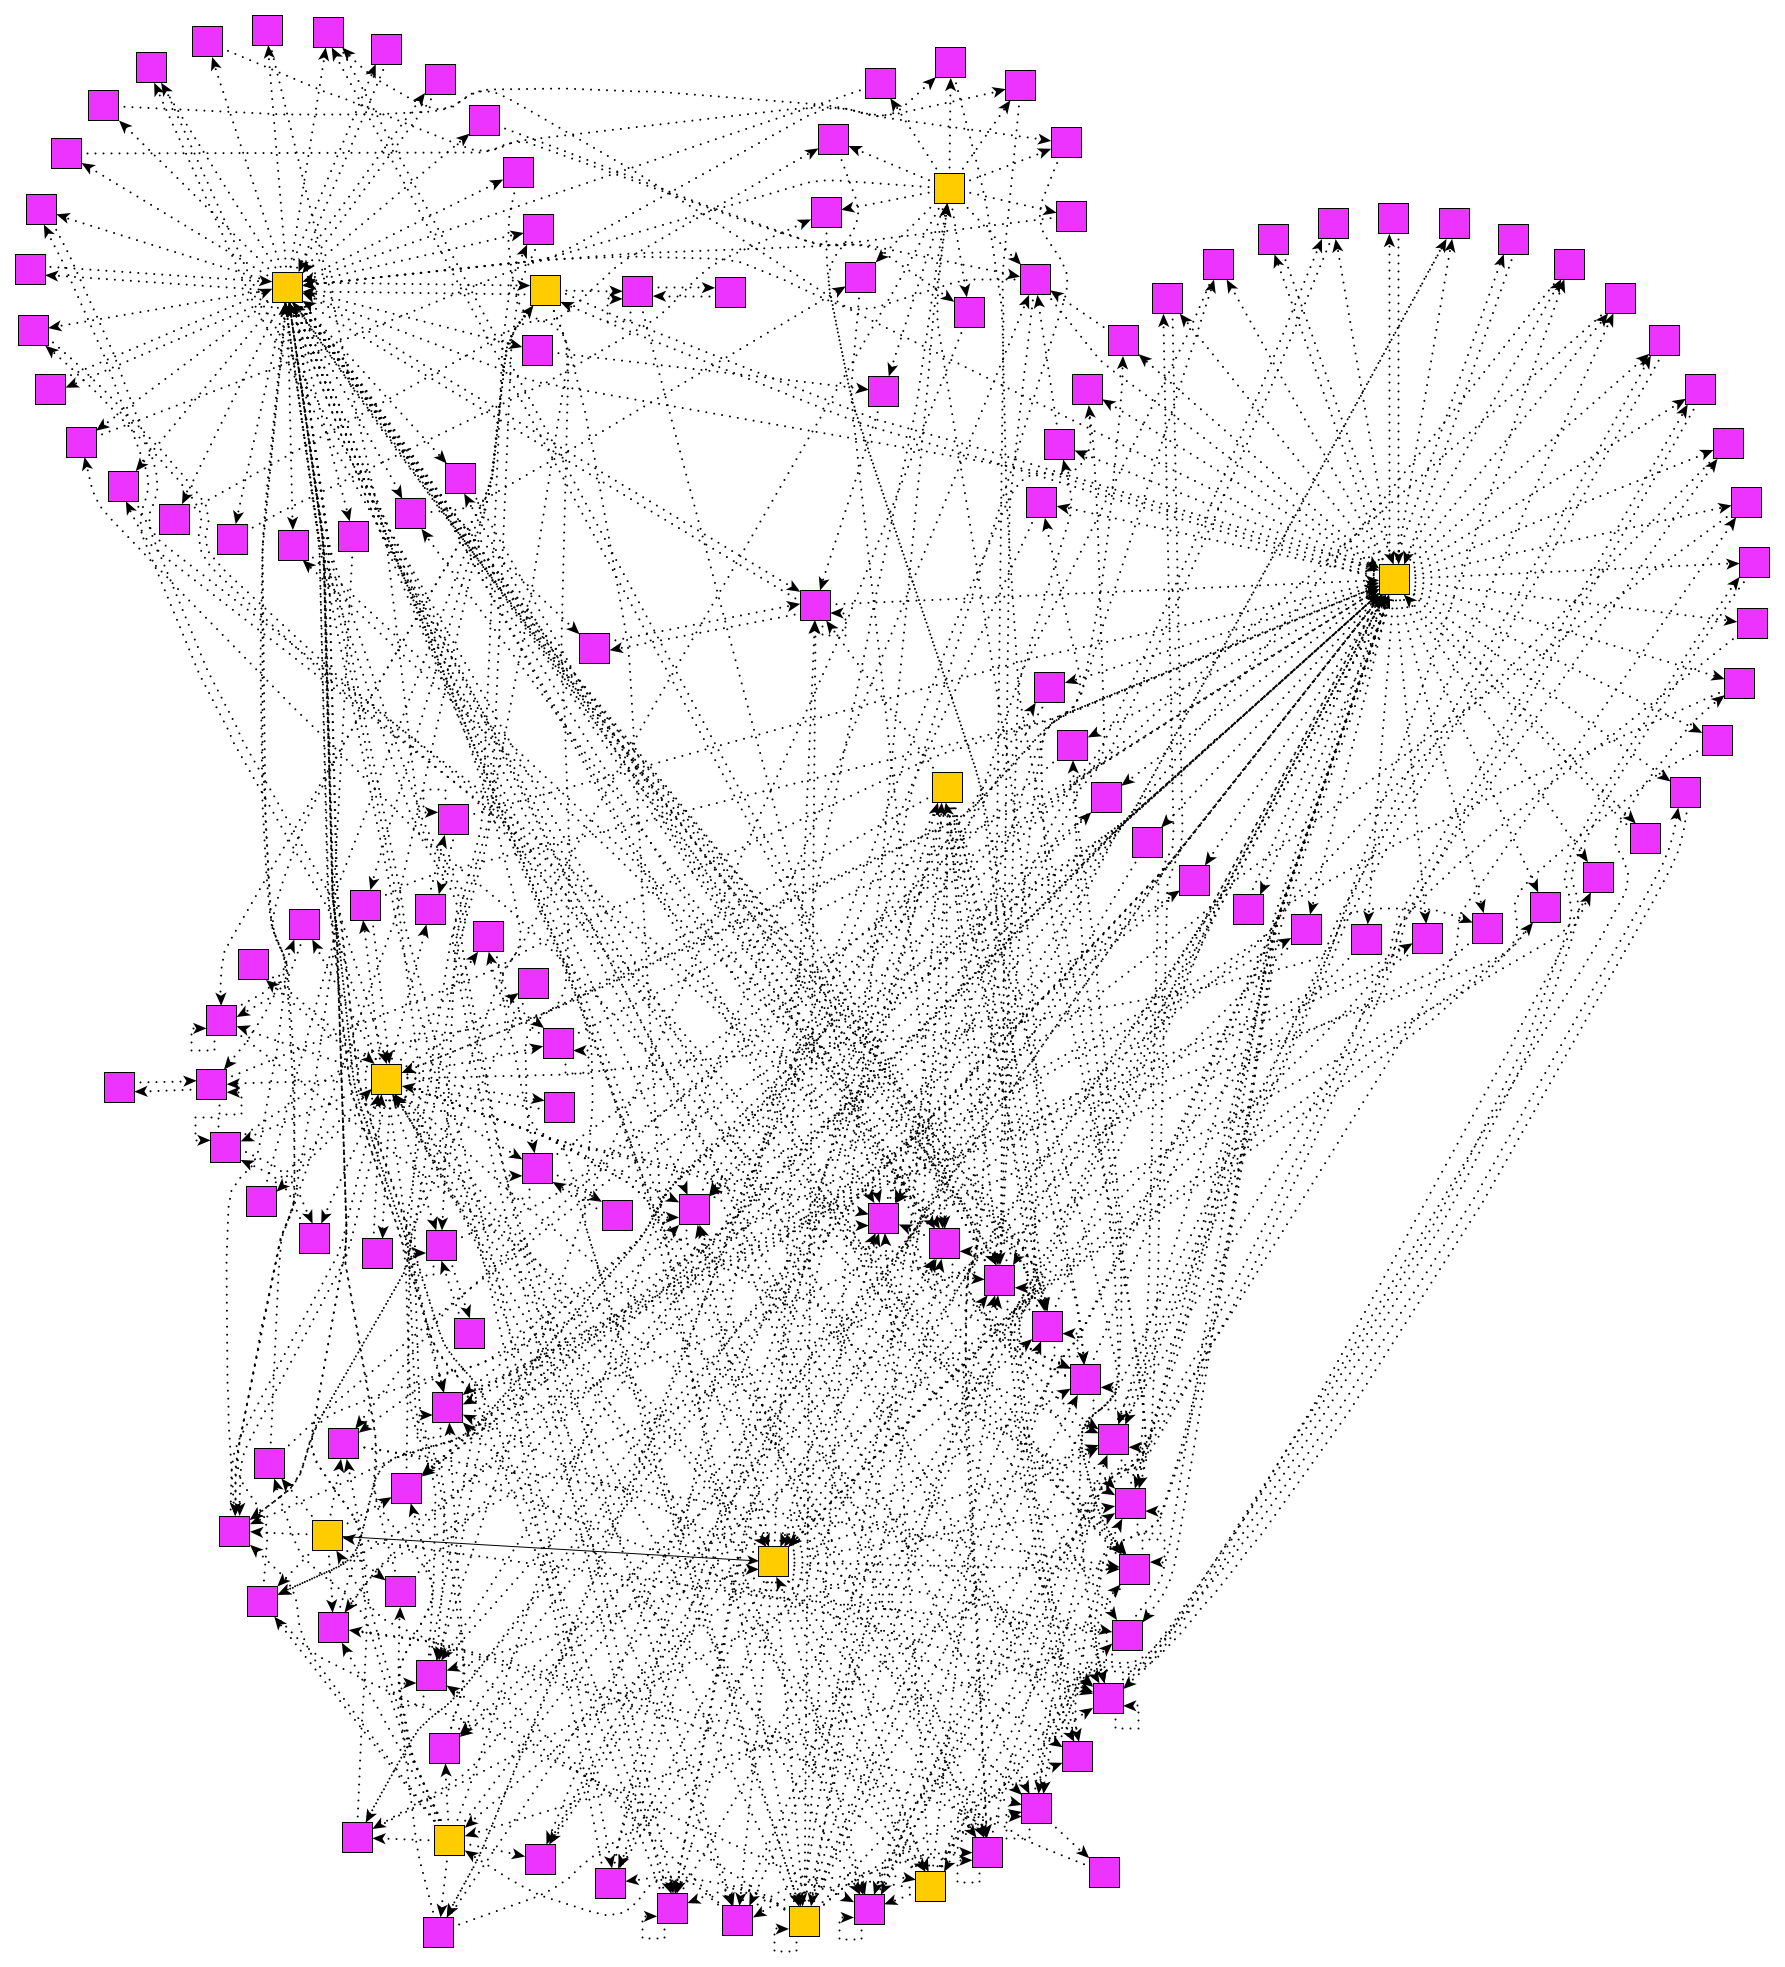
\includegraphics[width=\linewidth]{subfiles/imgs/balloon_ahb.png}
\caption{AHB Complete Automaton Clusterized}
\label{fig:AHB_balloon}
\end{figure}


\begin{table}[]
\centering
\caption{IMC Coverage Figures (\%)}
{\footnotesize
\begin{tabular}{|l|l|l|l|l|l|l|}
\hline
           & \multicolumn{3}{c|}{I2C} & \multicolumn{3}{c|}{AHB} \\ \hline
           & cov. & tot. & overall    & cov.  & tot. & overall \\ \hline
Overall    & 352     & 410  & 93.8\%    & 333   & 1057  & 61.3\%\\ \hline
block      & 164     & 180  & 95.4\%    & 51    & 68    & 85.55\% \\  \hline
Expression & 44      & 44   & 100\%     & 7     & 17    & 41.18\% \\ \hline
Toggle     & 112     & 148  & 75.68\%   & 266   & 963   & 30.17\% \\ \hline
FSM        & 32      & 38   & 83.36\%   & 9     & 9     & 100\%\\ \hline
\end{tabular}
}
\label{tab:cov_I2C}
\end{table}

Fault injection traces are then processed following rules described in section \ref{FBMC} extracting transitions probabilities between the connected subgraphs:


\begin{itemize}
    \item \texttt{Nominal 1} - Subgraph made of legal states only, part of the nominal execution.
    \item \texttt{Nominal 2} - Subgraph made of legal states only, part of the nominal execution.
    \item \texttt{Faulty  1} - Illegal state Subgraph, leading to a propagation of the fault to the output.
    \item \texttt{Faulty  2} - Illegal state Subgraph, leading to a simulation timeout.
\end{itemize}
The resulting model is represented on Fig. \ref{fig:simp_fsm}.

\begin{figure}[h]
    \centering



\tikzset{every picture/.style={line width=0.75pt}} %set default line width to 0.75pt        

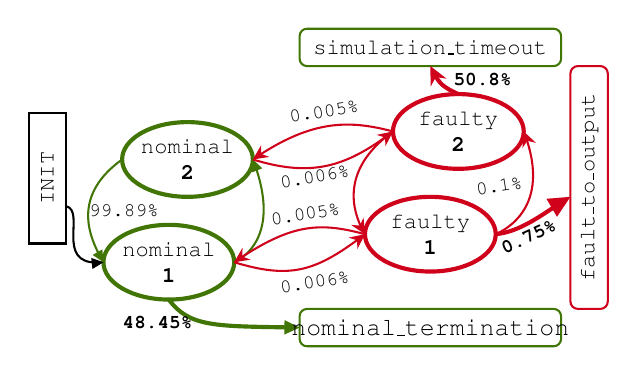
\begin{tikzpicture}[x=0.75pt,y=0.75pt,yscale=-0.9,xscale=0.9]
%uncomment if require: \path (0,300); %set diagram left start at 0, and has height of 300

%Rounded Diagonal Corner Rect [id:dp20075248017872083] 
\draw   (340,50) .. controls (340,50) and (340,50) .. (340,50) -- (360,50) .. controls (360,50) and (360,50) .. (360,50) -- (360,120) .. controls (360,120) and (360,120) .. (360,120) -- (340,120) .. controls (340,120) and (340,120) .. (340,120) -- cycle ;
%Shape: Ellipse [id:dp8528302096917133] 
\draw  [color={rgb, 255:red, 65; green, 117; blue, 5 }  ,draw opacity=1 ][fill={rgb, 255:red, 255; green, 255; blue, 255 }  ,fill opacity=0.28 ][line width=1.5]  (380,130) .. controls (380,118.95) and (395.67,110) .. (415,110) .. controls (434.33,110) and (450,118.95) .. (450,130) .. controls (450,141.05) and (434.33,150) .. (415,150) .. controls (395.67,150) and (380,141.05) .. (380,130) -- cycle ;
%Shape: Ellipse [id:dp18888957741575885] 
\draw  [color={rgb, 255:red, 208; green, 2; blue, 27 }  ,draw opacity=1 ][line width=1.5]  (535,60) .. controls (535,48.95) and (550.67,40) .. (570,40) .. controls (589.33,40) and (605,48.95) .. (605,60) .. controls (605,71.05) and (589.33,80) .. (570,80) .. controls (550.67,80) and (535,71.05) .. (535,60) -- cycle ;
%Rounded Rect [id:dp7596732624112932] 
\draw  [color={rgb, 255:red, 208; green, 2; blue, 27 }  ,draw opacity=1 ] (630,29) .. controls (630,26.79) and (631.79,25) .. (634,25) -- (646,25) .. controls (648.21,25) and (650,26.79) .. (650,29) -- (650,151) .. controls (650,153.21) and (648.21,155) .. (646,155) -- (634,155) .. controls (631.79,155) and (630,153.21) .. (630,151) -- cycle ;
%Curve Lines [id:da32583462836072785] 
\draw [color={rgb, 255:red, 208; green, 2; blue, 27 }  ,draw opacity=1 ][line width=1.5]    (626.45,97.16) .. controls (614.57,104.61) and (603.42,113.64) .. (590,115) ;
\draw [shift={(630,95)}, rotate = 149.68] [fill={rgb, 255:red, 208; green, 2; blue, 27 }  ,fill opacity=1 ][line width=0.08]  [draw opacity=0] (11.61,-5.58) -- (0,0) -- (11.61,5.58) -- cycle    ;
%Curve Lines [id:da3658243871665472] 
\draw    (376.92,130.2) .. controls (353.95,130.62) and (370.72,102.56) .. (360,100) ;
\draw [shift={(380,130)}, rotate = 173.77] [fill={rgb, 255:red, 0; green, 0; blue, 0 }  ][line width=0.08]  [draw opacity=0] (6.25,-3) -- (0,0) -- (6.25,3) -- cycle    ;
%Rounded Rect [id:dp11817172422118216] 
\draw  [color={rgb, 255:red, 65; green, 117; blue, 5 }  ,draw opacity=1 ] (621,155) .. controls (623.21,155) and (625,156.79) .. (625,159) -- (625,171) .. controls (625,173.21) and (623.21,175) .. (621,175) -- (489,175) .. controls (486.79,175) and (485,173.21) .. (485,171) -- (485,159) .. controls (485,156.79) and (486.79,155) .. (489,155) -- cycle ;
%Shape: Ellipse [id:dp43557254982651106] 
\draw  [color={rgb, 255:red, 65; green, 117; blue, 5 }  ,draw opacity=1 ][fill={rgb, 255:red, 255; green, 255; blue, 255 }  ,fill opacity=0.28 ][line width=1.5]  (390,75) .. controls (390,63.95) and (405.67,55) .. (425,55) .. controls (444.33,55) and (460,63.95) .. (460,75) .. controls (460,86.05) and (444.33,95) .. (425,95) .. controls (405.67,95) and (390,86.05) .. (390,75) -- cycle ;
%Shape: Ellipse [id:dp5343830480869827] 
\draw  [color={rgb, 255:red, 208; green, 2; blue, 27 }  ,draw opacity=1 ][line width=1.5]  (520,115) .. controls (520,103.95) and (535.67,95) .. (555,95) .. controls (574.33,95) and (590,103.95) .. (590,115) .. controls (590,126.05) and (574.33,135) .. (555,135) .. controls (535.67,135) and (520,126.05) .. (520,115) -- cycle ;
%Curve Lines [id:da2717718768343944] 
\draw [color={rgb, 255:red, 65; green, 117; blue, 5 }  ,draw opacity=1 ]   (450,130) .. controls (455.39,127.55) and (474.71,115.5) .. (460.89,77.37) ;
\draw [shift={(460,75)}, rotate = 428.82] [fill={rgb, 255:red, 65; green, 117; blue, 5 }  ,fill opacity=1 ][line width=0.08]  [draw opacity=0] (6.25,-3) -- (0,0) -- (6.25,3) -- cycle    ;
%Curve Lines [id:da23916036459047474] 
\draw [color={rgb, 255:red, 208; green, 2; blue, 27 }  ,draw opacity=1 ]   (590,115) .. controls (595.39,112.55) and (619.51,100.5) .. (605.88,62.37) ;
\draw [shift={(605,60)}, rotate = 428.82] [fill={rgb, 255:red, 208; green, 2; blue, 27 }  ,fill opacity=1 ][line width=0.08]  [draw opacity=0] (8.04,-3.86) -- (0,0) -- (8.04,3.86) -- (5.34,0) -- cycle    ;
%Curve Lines [id:da8274565221278805] 
\draw [color={rgb, 255:red, 208; green, 2; blue, 27 }  ,draw opacity=1 ]   (518.44,112.15) .. controls (511.34,98.05) and (509.91,78.08) .. (535,60) ;
\draw [shift={(520,115)}, rotate = 239.53] [fill={rgb, 255:red, 208; green, 2; blue, 27 }  ,fill opacity=1 ][line width=0.08]  [draw opacity=0] (8.04,-3.86) -- (0,0) -- (8.04,3.86) -- (5.34,0) -- cycle    ;
%Curve Lines [id:da4524486896686448] 
\draw [color={rgb, 255:red, 65; green, 117; blue, 5 }  ,draw opacity=1 ][line width=0.75]    (378.51,127.37) .. controls (370.77,113.26) and (364.78,93.17) .. (390,75) ;
\draw [shift={(380,130)}, rotate = 239.53] [fill={rgb, 255:red, 65; green, 117; blue, 5 }  ,fill opacity=1 ][line width=0.08]  [draw opacity=0] (6.25,-3) -- (0,0) -- (6.25,3) -- cycle    ;
%Curve Lines [id:da8065399762870671] 
\draw [color={rgb, 255:red, 208; green, 2; blue, 27 }  ,draw opacity=1 ]   (517.28,117.06) .. controls (492.7,135.43) and (479.11,138.85) .. (450,130) ;
\draw [shift={(520,115)}, rotate = 142.55] [fill={rgb, 255:red, 208; green, 2; blue, 27 }  ,fill opacity=1 ][line width=0.08]  [draw opacity=0] (8.04,-3.86) -- (0,0) -- (8.04,3.86) -- (5.34,0) -- cycle    ;
%Curve Lines [id:da3954387747286521] 
\draw [color={rgb, 255:red, 208; green, 2; blue, 27 }  ,draw opacity=1 ]   (532.26,62.06) .. controls (507.36,80.43) and (489.11,83.85) .. (460,75) ;
\draw [shift={(535,60)}, rotate = 142.55] [fill={rgb, 255:red, 208; green, 2; blue, 27 }  ,fill opacity=1 ][line width=0.08]  [draw opacity=0] (8.04,-3.86) -- (0,0) -- (8.04,3.86) -- (5.34,0) -- cycle    ;
%Curve Lines [id:da16071146130984038] 
\draw [color={rgb, 255:red, 208; green, 2; blue, 27 }  ,draw opacity=1 ]   (452.76,128.14) .. controls (482.07,108.67) and (496.88,108.86) .. (520,115) ;
\draw [shift={(450,130)}, rotate = 325.61] [fill={rgb, 255:red, 208; green, 2; blue, 27 }  ,fill opacity=1 ][line width=0.08]  [draw opacity=0] (8.04,-3.86) -- (0,0) -- (8.04,3.86) -- (5.34,0) -- cycle    ;
%Curve Lines [id:da2703895401851424] 
\draw [color={rgb, 255:red, 208; green, 2; blue, 27 }  ,draw opacity=1 ]   (462.78,73.14) .. controls (492.37,53.67) and (511.88,53.86) .. (535,60) ;
\draw [shift={(460,75)}, rotate = 325.61] [fill={rgb, 255:red, 208; green, 2; blue, 27 }  ,fill opacity=1 ][line width=0.08]  [draw opacity=0] (8.04,-3.86) -- (0,0) -- (8.04,3.86) -- (5.34,0) -- cycle    ;
%Curve Lines [id:da7497874187898392] 
\draw [color={rgb, 255:red, 65; green, 117; blue, 5 }  ,draw opacity=1 ][line width=1.5]    (480.42,164.92) .. controls (439.36,164.22) and (425.94,164.64) .. (415,150) ;
\draw [shift={(485,165)}, rotate = 181.07] [fill={rgb, 255:red, 65; green, 117; blue, 5 }  ,fill opacity=1 ][line width=0.08]  [draw opacity=0] (8.13,-3.9) -- (0,0) -- (8.13,3.9) -- cycle    ;
%Rounded Rect [id:dp7577300259636373] 
\draw  [color={rgb, 255:red, 65; green, 117; blue, 5 }  ,draw opacity=1 ] (621,5) .. controls (623.21,5) and (625,6.79) .. (625,9) -- (625,21) .. controls (625,23.21) and (623.21,25) .. (621,25) -- (489,25) .. controls (486.79,25) and (485,23.21) .. (485,21) -- (485,9) .. controls (485,6.79) and (486.79,5) .. (489,5) -- cycle ;
%Curve Lines [id:da08983874906696832] 
\draw [color={rgb, 255:red, 208; green, 2; blue, 27 }  ,draw opacity=1 ][line width=1.5]    (556.82,28.58) .. controls (559.85,34.34) and (561.83,36.34) .. (570,40) ;
\draw [shift={(555,25)}, rotate = 63.43] [fill={rgb, 255:red, 208; green, 2; blue, 27 }  ,fill opacity=1 ][line width=0.08]  [draw opacity=0] (9.91,-4.76) -- (0,0) -- (9.91,4.76) -- (6.58,0) -- cycle    ;

% Text Node
\draw (350,85) node  [font=\footnotesize,rotate=-270] [align=left] {{\fontfamily{pcr}\selectfont INIT}};
% Text Node
\draw (640,90) node  [font=\footnotesize,rotate=-270] [align=left] {{\fontfamily{pcr}\selectfont fault\_to\_output}};
% Text Node
\draw (555,165) node  [font=\footnotesize] [align=left] {{\fontfamily{pcr}\selectfont {\small nominal\_termination}}};
% Text Node
\draw (415,130) node  [font=\footnotesize] [align=left] {\begin{minipage}[lt]{37.003356000000004pt}\setlength\topsep{0pt}
\begin{center}
{\fontfamily{pcr}\selectfont nominal}\\{\fontfamily{pcr}\selectfont \textbf{1}}
\end{center}

\end{minipage}};
% Text Node
\draw (570,60) node  [font=\footnotesize] [align=left] {\begin{minipage}[lt]{32.101644pt}\setlength\topsep{0pt}
\begin{center}
{\fontfamily{pcr}\selectfont faulty}\\{\fontfamily{pcr}\selectfont \textbf{2}}
\end{center}

\end{minipage}};
% Text Node
\draw (425,75) node  [font=\footnotesize] [align=left] {\begin{minipage}[lt]{37.003356000000004pt}\setlength\topsep{0pt}
\begin{center}
{\fontfamily{pcr}\selectfont nominal}\\{\fontfamily{pcr}\selectfont \textbf{2}}
\end{center}

\end{minipage}};
% Text Node
\draw (555,115) node  [font=\footnotesize] [align=left] {\begin{minipage}[lt]{32.101644pt}\setlength\topsep{0pt}
\begin{center}
{\fontfamily{pcr}\selectfont faulty}\\{\fontfamily{pcr}\selectfont \textbf{1}}
\end{center}

\end{minipage}};
% Text Node
\draw (555,15) node  [font=\footnotesize] [align=left] {{\fontfamily{pcr}\selectfont simulation\_timeout}};
% Text Node
\draw (391,102.5) node  [font=\scriptsize] [align=left] {{\fontfamily{pcr}\selectfont 99.89\%}};
% Text Node
\draw (498.08,49.3) node  [font=\scriptsize,rotate=-350.99] [align=left] {{\fontfamily{pcr}\selectfont 0.005\%}};
% Text Node
\draw (493.08,84.3) node  [font=\scriptsize,rotate=-350.99] [align=left] {{\fontfamily{pcr}\selectfont 0.006\%}};
% Text Node
\draw (591.92,89.3) node  [font=\scriptsize,rotate=-350.99] [align=left] {{\fontfamily{pcr}\selectfont 0.1\%}};
% Text Node
\draw (493.08,140.7) node  [font=\scriptsize,rotate=-350.99] [align=left] {{\fontfamily{pcr}\selectfont 0.006\%}};
% Text Node
\draw (488.08,104.3) node  [font=\scriptsize,rotate=-350.99] [align=left] {{\fontfamily{pcr}\selectfont 0.005\%}};
% Text Node
\draw (583,32.5) node  [font=\scriptsize] [align=left] {{\fontfamily{pcr}\selectfont \textbf{50.8\%}}};
% Text Node
\draw (607.64,116.42) node  [font=\scriptsize,rotate=-335.61] [align=left] {{\fontfamily{pcr}\selectfont \textbf{0.75\%}}};
% Text Node
\draw (409,162.5) node  [font=\scriptsize] [align=left] {{\fontfamily{pcr}\selectfont \textbf{48.45\%}}};


\end{tikzpicture}
    \caption{Extracted FSM for the I2C Block}
    \label{fig:simp_fsm}
\end{figure} 


\subsection{AHB Block Modeling} \label{ahbinterfacetestcase}
The AHB bus interface is taken from the GRLIB \cite{GRLIB} library with added custom logic to connect it to the master parallel interface of the I2C. The added logic comprise an interpreter for the command received by the I2C and the glue logic interface to the AHB master side. A verification IP is connected to the AHB slave interface side to respond to transactions and check protocol. Fig. \ref{fig:chronogluewrite} represents the translation of I2C signals into an AHB transaction by the system. Coverage for AHB block is low and can be explained as only a limited use of the AHB protocol is made:
\begin{enumerate}
    \item only byte accesses are performed.
    \item only single (SINGLE) non-sequential (NONSEQ) transfers are performed.
    \item the VIP has not been programmed to insert HREADY wait states in the transaction.
    \item the VIP has not be programmed to generate HRESP transaction response error.
\end{enumerate}
The low coverage obtained here doesn't restrict the generality of the methodology but may prevents some failure modes to be identified in this specific case.

%\begin{table*}[]
%\centering
%\caption{Block and Full System Fault Injection Results}
%{\footnotesize
%\begin{tabular}{|ll|l|l|ll|}
%\hline
%\multicolumn{2}{|l|}{}                                           & I2C            & AHB             & \multicolumn{2}{c|}{I2C + AHB}                         \\ \hline
%\multicolumn{2}{|l|}{Golden states (static)}                     & 44             & 11              & \multicolumn{1}{l|}{44}              & 11              \\ \hline
%\multicolumn{2}{|l|}{Golden transitions (static)}                & 90             & 20              & \multicolumn{1}{l|}{89}              & 19              \\ \hline
%\multicolumn{2}{|l|}{Faulty states (static)}                     & 223            & 126             & \multicolumn{1}{l|}{198}             & 193             \\ \hline
%\multicolumn{2}{|l|}{Faulty transitions (static)}                & 1093           & 470             & \multicolumn{1}{l|}{899}             & 428             \\ \hline
%\multicolumn{2}{|l|}{Injected faults (400 / FF)}                 & 11670          & 41200           & \multicolumn{2}{c|}{52878}                             \\ \hline
%\multicolumn{1}{|l|}{\multirow{}{}{Detected faults}}  & golden & 6840 (58.61\%) & 19285 (46.80\%) & \multicolumn{1}{l|}{23840 (45.08\%)} & 22089 (41.77\%) \\ \cline{2-6} 
%\multicolumn{1}{|l|}{}                                  & faulty & 19 (0.16\%)    & 466 (1.31\%)    & \multicolumn{1}{l|}{219 (0.41\%)}    & 1970 (3.72\%)   \\ \hline
%\multicolumn{1}{|l|}{\multirow{}{}{Detecting states}} & golden & 44 (100\%)     & 11 (100\%)      & \multicolumn{1}{l|}{44 (100\%)}      & 11 (100\%)      \\ \cline{2-6} 
%\multicolumn{1}{|l|}{}                                  & faulty & 5 (1.87\%)     & 13 (9.48\%)     & \multicolumn{1}{l|}{5 (2.06\%)}      & 70 (34.31\%)    \\ \hline
%\end{tabular}
%}
%\label{block_full_system_fi_results}
%\end{table*}

\subsection{Complete System Test Case} \label{complete_test_case}
The complete system is composed of both the I2C slave and AHB master along with VIPs at both ends. As previously mentioned, probes are placed on all outputs of the complete system, leaving this time, faults freely propagating internally between the I2C and the AHB without being reported by FSV nor the simulation to be stopped. The main difference of this testbench regarding the two standalone previous ones is that faults injected in one block will be able to propagate to the other one (I2C $\rightarrow$ AHB, for example) and back-propagate to the first block (AHB $\rightarrow$ I2C) as simulation will not be stopped when the fault will output from the first (i.e. I2C), and later second (i.e. AHB), block. Such "fault loop" (I2C $\circlearrowleft$ AHB or AHB $\circlearrowleft$ I2C) are expected to be the main possible source of faulty states differences between the standalone and full system faulty states extraction. However, as faults are injected on the inputs in both approach (standalone and full system), we expect to capture, at least a part of theses "fault loops" induced faulty states in the standalone extractions, if such case exist.

The AltaRica structural model architecture follows the natural hierarchy of the system. As shown on Fig. \ref{fig:i2cahb}, the AltaRica models includes the exact same blocks with the same interconnections between blocks as the functional model.  The main I2C and AHB modules are composed of two sub-elements, shown respectively in Fig. \ref{fig:i2caps} and Fig. \ref{fig:ahbaps}. 

\begin{figure}[!h]
    \centering
    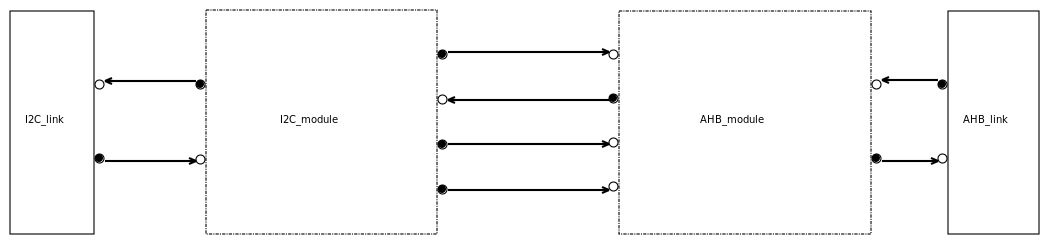
\includegraphics[width=\linewidth]{subfiles/imgs/I2C_AHB.png}
    \caption{I2C to AHB System Model}
    \label{fig:i2cahb}
\end{figure}
\begin{figure}[!h]
    \centering
    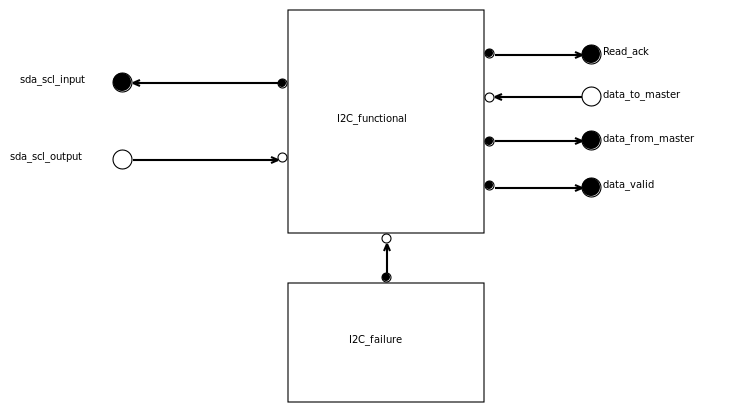
\includegraphics[width=\linewidth]{subfiles/imgs/I2C_module.png}
    \caption{I2C Block Model}
    \label{fig:i2caps}
\end{figure}
\begin{figure}[!h]
    \centering
    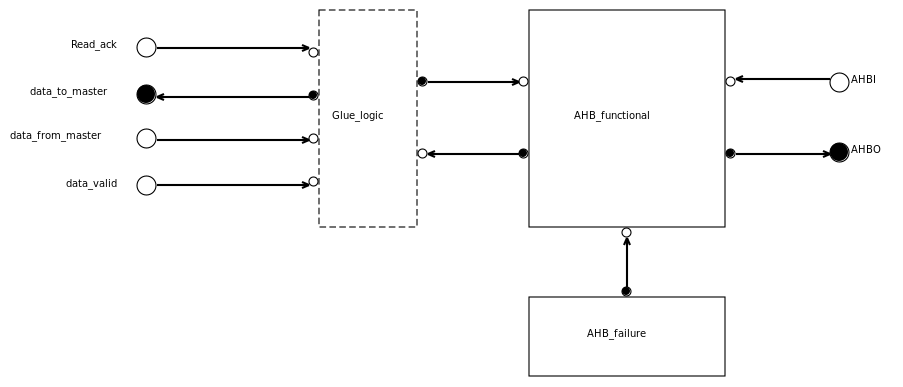
\includegraphics[width=\linewidth]{subfiles/imgs/AHB_module.png}
    \caption{AHB Block Model}
    \label{fig:ahbaps}
\end{figure}
The first element is the {\it functional} state machine of the module. In case of internal or external fault, this state machine will dispatch the fault to the impacted outputs. This state machine only model the internal faults propagation and do not generate any random failure on its own. The second element is the {\it internal failure} state machine. This state machine generate internal random failures and provide to the functional state machine the outputs impacted by it. 
In addition, the AHB module include an additional glue-logic block that converts I2C output signals to AHB bridge input signals. No internal failure are generated by this element. 
At both end of the I2C and AHB blocks, links module have been added to model the faults coming from outside of the system. To model the behavior of the I2C and AHB system, only standalone block fault injection test results have been used.

Depending on the methodology, two types of metrics can be extracted. The first one is the probability to propagate internal failure to one or more outputs of the system. From the test results, this probability has been extracted by considering all faults injected in the studied system. The probability to propagate internal faults to an output of the system is then equal to the ratio between the faults detected by the output probe and the total number of faults injected.

The second metrics is the probability to propagate a failure from an input of the system to one or more output of the system. For this metric, only fault injected on inputs have been taken into account. This probability is the ratio of the input faults leading to an erroneous output over the total number of input faults injected.

SimfiaNeo allows to perform Monte-Carlo simulation. In this type of simulation, a large number of failure scenarios are generated to assess the mean behavior of the system under random failure scenarios. 
The first possible assessment randomly injected one failure by failure scenario inside the system while the outputs are monitored. If at least one output triggers a faulty state, the error is accounted to have been propagated outside of the system. With this methodology, it’s possible to estimate the probability to have a failure propagation from the I2C+AHB system to the I2C or AHB external signals. 
The second possible assessment randomly injected one failure by failure scenario in a link module and monitored the other link module. If the opposite link module triggers a faulty state, the error is accounted to have been propagated from one end to another. With this methodology, it is possible to estimate the probability to have a failure propagation from AHB or I2C back to the other link.

\section{Results on the $I2C$ to $AHB$ System}
Result of composition obtained by SimfiaNeo are compared to fault injection performed on the full system with probes set only on external outputs of the system on table \ref{results_ahb_i2c} for the I2C and AHB side signal. Because the system is simple and faults propagate only forward, it came to simple probability multiplication explaining exact matching of model and system fault injection. No back-propagating faults were observed.

%\begin{table}[]
%\caption{AHB Block Fault Injection Vs Altarica Model Failures}
%{\footnotesize
%\begin{tabular}{|l|l|l|}
% \hline
%AHB failure & I2C+AHB & Model   \\ \hline
%haddr       & 0.00551 & 0.00551 \\ \hline
%hwdata      & 0.00382 & 0.00382 \\ \hline
%hsize       & 0.00068 & 0.00068 \\ \hline
%hbusreq     & 0.00026 & 0.00026 \\ \hline
%hwrite      & 0.00022 & 0.00022 \\ \hline
%\end{tabular}
%}
%\label{results_ahb}
%\end{table}
%\begin{table}[]
%\caption{I2C Block Fault Injection Vs Altarica Model Failures}
%{\footnotesize
%\begin{tabular}{|l|l|l|}
% \hline
%I2C Failure & I2C+AHB & Model   \\ \hline
%SDA         & 0.00338 & 0.00339 \\ \hline
%Read req    & 0.00254 & 0.00255 \\ \hline
%Data        & 0.00580 & 0.00581 \\ \hline
%Data valid  & 0.00322 & 0.00323 \\ \hline
%\end{tabular}
%}
%\label{results_i2c}
%\end{table}

\begin{table}[H]
\caption{RTL Fault Injection Vs Altarica Model Failures}
{\footnotesize
\begin{tabular}{|l|l|l|l|l|l|}
\hline
\multicolumn{1}{|c|}{AHB} & \multicolumn{1}{c|}{I2C+AHB} & \multicolumn{1}{c|}{Altarica} & \multicolumn{1}{c|}{I2C} & \multicolumn{1}{c|}{I2C+AHB} & \multicolumn{1}{c|}{Altarica} \\
\multicolumn{1}{|c|}{Failure} & \multicolumn{1}{c|}{RTL} & \multicolumn{1}{c|}{Model} & \multicolumn{1}{c|}{Failure} & \multicolumn{1}{c|}{RTL} & \multicolumn{1}{c|}{Model} \\ \hline
haddr & 0.00551 & 0.00551 & SDA & 0.00338 & 0.00339 \\ \hline
hwdata & 0.00382 & 0.00382 & Read req & 0.00254 & 0.00255 \\ \hline
hsize & 0.00068 & 0.00068 & Data & 0.00580 & 0.00581 \\ \hline
hbusreq & 0.00026 & 0.00026 & Data valid & 0.00322 & 0.00323 \\ \hline
hwrite & 0.00022 & 0.00022 &  &  &  \\ \hline
\end{tabular}
}
\label{results_ahb_i2c}
\end{table}


\section{Second Proof of Concept 4BlocksSystem}

\section{Discussion and Future Work}
\label{sec:discussion}
In this work, we have proposed and experimented the use of Model-Based Safety Assessment on digital system for safety analysis. We have addressed the construction of dysfunctional model for digital system using simulation and have been able to build a simple, but functional dysfunctional model in Altarica. Ongoing work include automatic dysfunctional models reduction to more than one state and the application to a small RISCV SoC and software reliability\cite{iolts2022}.


